\RequirePackage{silence}
\WarningFilter{hyperref}{Token not allowed}
\WarningFilter{microtype}{tracking amount}
\WarningFilter{chessfss}{\comment already}
\documentclass[xcolor={x11names,svgnames,dvipsnames},trans]{beamer}
\usepackage{pgfpages}
\usepackage{qrcode}
\usepackage[british]{babel}

%% Glossy pretty look for the presentation and transparency (w/o overlays and animations) versions!
\mode<beamer|trans>{
\useoutertheme[glossy]{wuerzburg}
\useinnertheme[shadow,outline]{chamfered}
\usecolortheme{shark}
}
\setbeamertemplate{navigation symbols}{}
\setbeamertemplate{frametitle continuation}[from second][(cont'd)]
\usefonttheme[stillsansseriftext,stillsansserifsmall]{serif}

%% Save up on ink for the 4-up handouts
\mode<handout>{
\useoutertheme{wuerzburg}
\useinnertheme[outline]{chamfered}
%\pgfpagesuselayout{4 on 1}[a4paper, landscape, border shrink=10mm]
\pgfpagesuselayout{2 on 1}[a4paper, border shrink=10mm]
\pgfpageslogicalpageoptions{1}{border code=\pgfstroke}
\pgfpageslogicalpageoptions{2}{border code=\pgfstroke}
%\pgfpageslogicalpageoptions{3}{border code=\pgfstroke}
%\pgfpageslogicalpageoptions{4}{border code=\pgfstroke}
\setbeamercolor{structure}{fg=black}
\setbeamercolor{alerted text}{fg=black}
}

\mode<presentation>{\AtBeginSection[]{%
\begin{frame}
\frametitle{Contents}
\tableofcontents[currentsection]
\end{frame}}}
\usepackage[T1,safe]{tipa}
\usepackage{microtype}
\usepackage[utf8]{inputenc}
\usepackage[T1]{fontenc}
\usepackage{libertine}
\usepackage[scaled=.77]{beramono}
\SetTracking{encoding=*}{-39}
\usepackage{relsize,tabularx}
\usepackage{hologo,textcomp}
\usepackage{comment}
\usepackage[skaknew]{chessboard,skak}
\usepackage{multicol,booktabs}
\usepackage{listings}
\lstset{upquote,keepspaces=true,columns=spaceflexible,
basicstyle=\ttfamily\scriptsize,%
breaklines=true,breakindent=0pt,xleftmargin=0pt, xrightmargin=6pt,%
language=[LaTeX]TeX, texcsstyle=*\bfseries\color{Maroon}, commentstyle=\sffamily\itshape\smaller\color{SeaGreen4},
emphstyle=\bfseries\color{RoyalBlue3},escapechar={:},
emphstyle={[2]{\bfseries\color{Sienna2}}},
postbreak=\mbox{{\smaller\color{gray}$\hookrightarrow$}}
}
\mode<handout>{
   \lstset{
   texcsstyle=*\bfseries, commentstyle=\sffamily\itshape\smaller,
   emphstyle=\bfseries,escapechar={:},
   emphstyle={[2]{\bfseries}},
   emphstyle={[3]{\bfseries}},
   postbreak=\mbox{{\smaller$\hookrightarrow$}}
   }
}
\makeatletter
\lst@CCPutMacro\lst@ProcessOther {"2D}{\lst@ttfamily{-{}}{-{}}}
\@empty\z@\@empty
\makeatother
\usepackage{tikz}
\usepackage{pgfgantt}
\usetikzlibrary{shapes,arrows,positioning,matrix,chains,fit}
\usetikzlibrary{backgrounds}
\usepackage{multicol,multirow}
\usepackage[version=3]{mhchem}
\usepackage{chemfig}
\usepackage{expex,qtree}
\usepackage{texshade}
\usepackage[detect-all]{siunitx}
\usepackage[siunitx]{circuitikz}
\usepackage{smartdiagram}
\usepackage{bytefield}
% \usepackage{pstricks,pst-barcode}
% \usepackage{auto-pst-pdf}
\usepackage{pgfplots}
\pgfplotsset{compat=1.12}
\usepackage{cwpuzzle}
\usepackage{gchords,guitar}
\usepackage{spreadtab}
\usepackage{ccicons}
\usepackage{marvosym}
\usepackage{upgreek}
\usepackage{adforn}
% \ifpdf
\pdfmapfile{+webo.map}
% \fi
\newcommand{\wb}[1]{{\usefont{U}{webo}{xl}{n}#1}}
\usepackage{bookmark}
\setlength\fboxsep{0pt}
\author[Sa\'ul D\'iaz Infante Velasco]{
    \texorpdfstring{
        Sa\'ul D\'iaz Infante Velasco
        (\url{sauldiazinfante@gmail.com})
        \\
        \url{http://liantze.penguinattack.org}}
        {LianTze Lim (Ph.D.)}
    }
\title{
    EXISTENCE, CHARACTERIZATION AND SIMULATION OF OPTIMAL
    POLICIES IN A FAMILY OF EPIDEMIC MODELS}
\subtitle{\texorpdfstring{(\textsc{first presented at mosc}\oldstylenums{2011})\\%
\hrulefill\ \adforn{57}\thickspace\wb{m}\thickspace\adforn{29}\ \hrulefill}{First Presented at MOSC 2011; some modifications since}}
\date[\ccbyncsa]{\ccbyncsa\ (Yes, you can reuse this deck \Smiley)}
\titlegraphic{
\includegraphics[width=.3\textwidth]{TFZsuperellipse-crop}\\\tiny Illustration by Duane Bibby}

\hypersetup{%
pdfauthor={LianTze Lim}, %% the "author" field from above includes garbage code...
pdfkeywords={latex,features,publicity,preview}
}

\begin{document}
\begin{frame}[plain]
\maketitle
\end{frame}

\begin{frame}
\frametitle{Contents}
\tableofcontents
\end{frame}


% !TEX root=talk.tex
\section[Introduction]{What are \TeX, \LaTeX\ and Friends?}

\begin{frame}

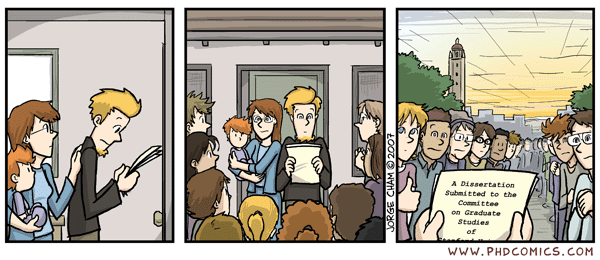
\includegraphics[width=.53\textwidth]{phdcomics-submission01}\par
\pause{\centering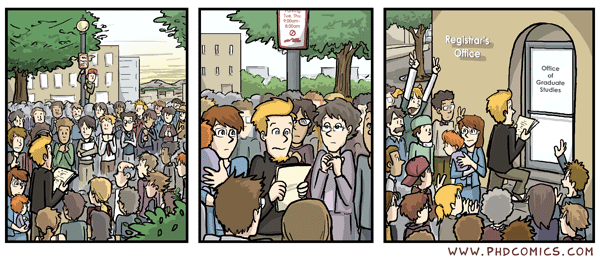
\includegraphics[width=.53\textwidth]{phdcomics-submission02}\par}
\pause{\fontfamily{augie}\small\selectfont PHD Comics by Jorge Cham}\hfill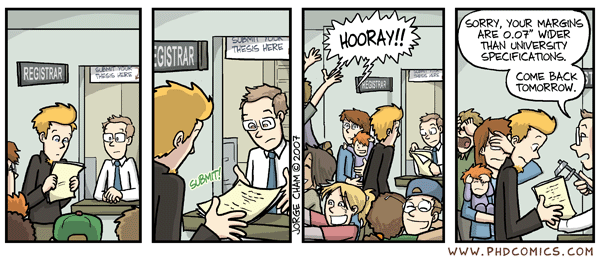
\includegraphics[width=.53\textwidth]{phdcomics-submission03}

\end{frame}


\begin{frame}
\frametitle{Ever Worried about These?}
\begin{itemize}
\item<2-16> Is my literature survey strong enough?
\item<3-15,17|alert@17|trans:alert@1|handout:alert@1> My bibliography/citation formatting got inconsistent.
\item<4-15,17|alert@17|trans:alert@1|handout:alert@1> My citation and bibliography aren't synchronised!
\item<5-15,17|alert@17|trans:alert@1|handout:alert@1> My math equations don't display/print correctly.
\item<6-16> Should this discussion go under this section or that?
\item<7-15,17|alert@17|trans:alert@1|handout:alert@1> What formatting did I use for my subsection headings again?
\item<8-15,17|alert@17|trans:alert@1|handout:alert@1> Didn't I set that heading to bold and italic 5 minutes ago?
\item<9-15,17|alert@17|trans:alert@1|handout:alert@1> My section/figure/page numbering's gone all wrong!
\item<10-16> Does this subsection go together with this section?
%\item<alert@2> My page numbering's gone all wrong!
\item<11-15,17|alert@17|trans:alert@1|handout:alert@1> Oops, I forgot to update the TOC.
\item<12-16> What results should I put in this table?
%\item<13-16,18|alert@18> How do I fit/split this huge table on/across page(s)?
\item<13-15,17|alert@17|trans:alert@1|handout:alert@1> My figure jumped off the page again!
\item<14-15,17|alert@17|trans:alert@1|handout:alert@1> The application crashed!
\item<15-15,17|alert@17|trans:alert@1|handout:alert@1> \textbf{MY FILE GOT CORRUPTED!!!}
\end{itemize}
\end{frame}

\begin{frame}<1>[label=texNfriends]
\frametitle{What are \TeX\ and \LaTeX,\ and Friends?}

\begin{description}
\item<1>[\TeX] 
\begin{itemize}
\item From Greek $\uptau\upepsilon\upchi$
\item \textsmaller{ASCII} \texttt{TeX}, \textsmaller{\textipa{/tEx/}, \textipa{/tEk/}}
\item A \structure{computer typesetting system} created by Donald Knuth
\item for `the creation of beautiful books'
\end{itemize}


\item<2>[\LaTeX]
\begin{itemize}
\item \textsmaller{ASCII} \texttt{LaTeX}, \textsmaller{\textipa{/"leItEx/}, \textipa{/"leItEk/}, \textipa{/"lA:tEx/}, \textipa{/"lA:tEk/}}
\item A \structure{document preparation system} by Leslie Lamport
	\end{itemize}

\pause

\item<3-4>[Binaries]
	\begin{itemize}
  \item \structure{\hologo{eTeX}}: additional primitives to \hologo{TeX}
	\item \structure{\alert<4>{\hologo{pdfTeX}}}: additional PDF-related primitives
  \item \structure{Xe\TeX}: native UTF-8 input; can access system fonts
	\item \structure{\hologo{LuaTeX}}: includes the Lua scripting engine
\end{itemize}
\item <5>[Friends]
\begin{itemize}
\item \structure{Bib\TeX}, \structure{MakeIndex}, \structure{METAFONT}, \structure{METAPOST},  \ldots
\item \url{http://www.ctan.org/what_is_tex.html}
\end{itemize}
\end{description}
\end{frame}

{\setbeamertemplate{background canvas}{\hskip-2em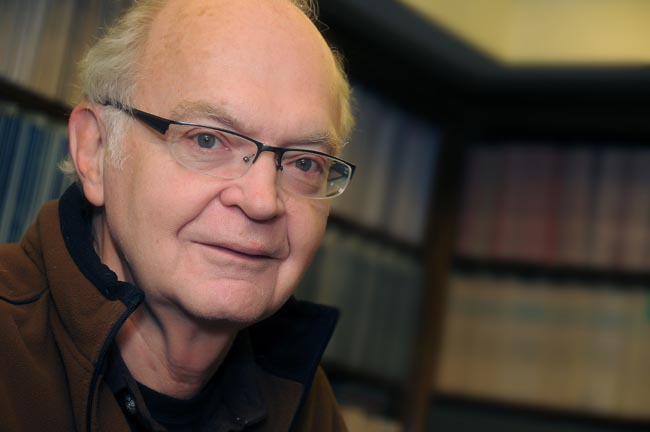
\includegraphics[height=\paperheight]{d_knuth_noticia}}
\setbeamercolor{itemize item}{fg=structure.fg!45}
\begin{frame}[plain,t]
\vfill
\hfill
\begin{minipage}{.42\textwidth}
\usebeamercolor[bg]{normal text}
\hspace{1em}\textbf{\large Donald Knuth (1938--)}
\begin{itemize}
\usebeamercolor[bg]{normal text}
\item American computer scientist, mathematician, and professor emeritus at Stanford University
\item Author of the multi-volume work The Art of Computer Programming
\item ``Father of the analysis of algorithms''
\end{itemize}
\end{minipage}

\bigskip

\begin{quote}
\usebeamercolor[bg]{normal text}
``Science is what we understand well enough to explain to a computer. Art is everything else we do.''

\medskip

``If you optimize everything, you will always be unhappy.''
\end{quote}
\vspace*{-4\baselineskip}\null
\end{frame}}

\mode<beamer>{
  \againframe<2>{texNfriends}
}

{\setbeamertemplate{background canvas}{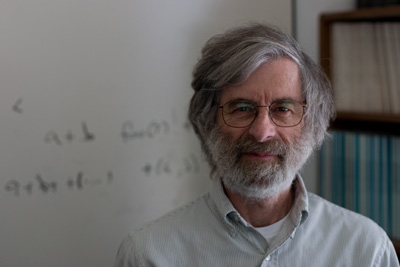
\includegraphics[height=\paperheight]{lamport}}
\setbeamercolor{itemize item}{fg=structure.fg!45}
\begin{frame}[plain,t]
\vfill
\begin{minipage}{.45\textwidth}
\usebeamercolor[bg]{normal text}
\hspace{1em}\textbf{\large Leslie Lamport (1941--)}
\begin{itemize}
\usebeamercolor[bg]{normal text}
\item American computer scientist
\item Laid the foundations of the theory of distributed systems
\end{itemize}

\bigskip

\begin{quote}
\usebeamercolor[bg]{normal text}
``A distributed system is one in which the failure of a computer you didn't even know existed can render your own computer unusable.''\end{quote}
\end{minipage}
\end{frame}
}

\mode<beamer>{
  \againframe<3->{texNfriends}
}

\begin{frame}
\frametitle{Why?}
\framesubtitle{From \url{http://www.ctan.org/what_is_tex.html}}
\begin{columns}[T]
\begin{column}{.46\textwidth}
\begin{block}{Output Quality}
\begin{itemize}
\item It has the best output.
\item It knows typesetting.
\end{itemize}
\end{block}

\begin{block}{Superior Engineering}
\begin{itemize}
\item It's fast.
\item It's stable.
\item It's not rigid (extensible).
\item Plain text input.
\item Many output types.
\end{itemize}
\end{block}
\end{column}

\begin{column}{.46\textwidth}
\begin{block}{Freedom}
\begin{itemize}
\item It's free.
\item It runs anywhere.
\end{itemize}
\end{block}

\begin{block}{Popularity}
\begin{itemize}
\item It's the standard (in academia and science).
\end{itemize}
\end{block}
\end{column}
\end{columns}
\end{frame}

\begin{frame}
\frametitle{Typesetting and Word Processing}
\framesubtitle{Apples and Oranges}
\begin{itemize}
\item<+-> Word processors
\begin{itemize}
\item Replacement of mechanical typewriters
\item Word, OpenOffice, AbiWord, \ldots
\end{itemize}
\item<+-> Typesetting and Desktop publishing
\begin{itemize}
\item For publication and printing
\item InDesign, QuarkXPress, Scribus\ldots
\end{itemize}
\end{itemize}
\end{frame}

\begin{frame}
\frametitle{Scalability}

\centering
\begin{tikzpicture}
%\draw[help lines,gray!20] (0,0) grid (6,4);
%\draw[semithick] (0,0) rectangle (6,4);
\draw[semithick,->,>=latex'] (-.5, 0) -- (6.5, 0);
\draw[semithick,->,>=latex'] (0, -.5) -- (0,5);
\draw[dashed,structure.fg!50!black,semithick] (0, 0.2) parabola (3.5,4) node[above,font=\footnotesize,text=black]{impossible to do} (3.5, 4);
\node[left] at (3,3) {Word$\textsuperscript{\textregistered}$};
\draw[structure.fg!50!black,semithick] (0, 1) parabola (6,3); 
\node at (5.2,2) {\LaTeX};
\node[below,font=\footnotesize] at (3,0) {document complexity and size};
\node[xshift=-8pt,yshift=4pt,font=\footnotesize,transform shape,rotate=90] at (0,2.2) {effort and time consumption};
\end{tikzpicture}

{\small Scalability of \LaTeX\ and Microsoft Word\textregistered\ against document size and complexity (redrawn from Marko Pinteric's original at \url{http://www.pinteric.com/miktex.html})}



\end{frame}

\begin{frame}
\frametitle{Professional Typesetting Quality Output}
\setlength\fboxsep{.25em}

\begin{itemize}
%\item Follows typography best practice
\item<+-> Typesetting quality and legibility
\begin{itemize}
\item good kerning hinting and correct ligatures
\item inter-word, line and paragraph spacing
\item context-sensitive hyphenation
\end{itemize}
%
\begin{columns}[T]
\begin{column}{.48\linewidth}
\fcolorbox{black}{white}{
\begin{minipage}{.98\linewidth}
\centering\large\fontfamily{qtm}\selectfont \alert{Ta}ble \alert{fi}ery \alert{fl}u\alert{ff}y\par
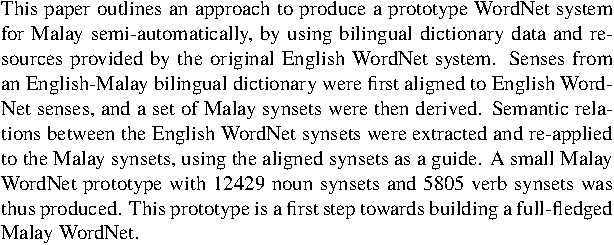
\includegraphics[width=\linewidth]{examples/latex-text-sample}
\end{minipage}}
\end{column}
\begin{column}{.48\linewidth}
\fcolorbox{black}{white}{
\begin{minipage}{.98\linewidth}
\centering\large
\includegraphics[height=.95em]{examples/word-ligature-cropped}\par
\vspace*{-1pt}\onslide<1>{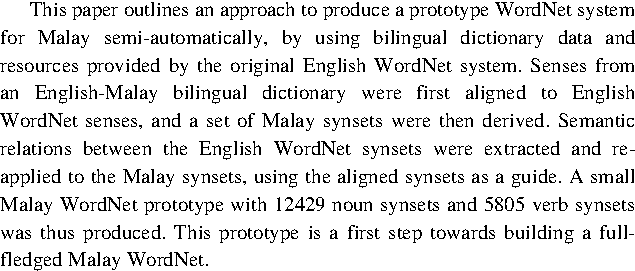
\includegraphics[width=.98\linewidth]{examples/word-text-nohyph-cropped}}\onslide<2-|trans:0|handout:0>{\llap{\setlength\fboxsep{0pt}\colorbox{white}{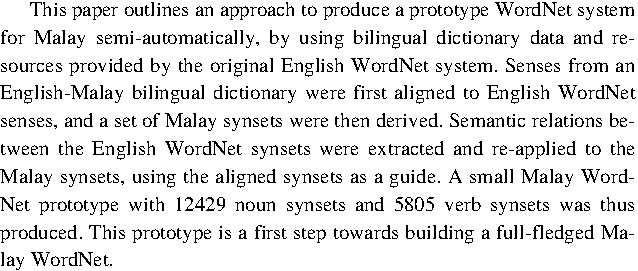
\includegraphics[width=.98\linewidth]{examples/word-text-hyph-cropped}}}}
\end{minipage}}
\end{column}
\end{columns}

\medskip

\item<3-> Correct mathematical typesetting (spacing etc)

\begin{columns}[T]
\begin{column}{.48\linewidth}
\fcolorbox{black}{white}{
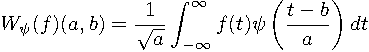
\includegraphics[width=.98\linewidth]{examples/latex-math-sample-cropped}}
\end{column}
\begin{column}{.48\linewidth}
\onslide<3>{\fcolorbox{black}{white}{
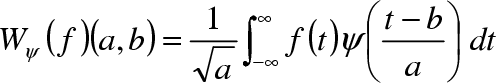
\includegraphics[width=.94\linewidth]{examples/eq-word}}}%
\onslide<4|trans:0|handout:0>{\llap{\fcolorbox{black}{white}{
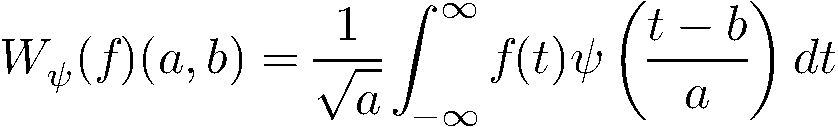
\includegraphics[width=.94\linewidth]{examples/word2010-maths-cropped}}}}
\end{column}
\end{columns}

\end{itemize}
\end{frame}

\begin{frame}
\frametitle{Where Would I Want to Use \hologo{LaTeX}?}
\begin{itemize}
\item Beautiful typographic output \pause(OK not everyone cares that much\ldots)
\item Documents with complex structures
\item Lots of mathematics \pause(or other specific needs)\pause
\item When publishers \alert{require} them
\item Batch processing of data into reports, etc.
\pause
\item Back-end of other applications
\end{itemize}
\end{frame}

%\begin{frame}
%\frametitle{Some Cons}
%\begin{itemize}
%%  \item Usually not WYSIWYG (except commercial solutions)
%  \item Initial learning curve (that's what I'm here for)
%%  \item Hard to produce ``flashy'' docs (with too many fonts, colours\ldots)
%  \item Overkill for simple documents
%  \item Not as suitable for graphic-intensive material (e.g.\ advertising)
%%  \item Not so good for advertisements, etc
%\end{itemize}
%\end{frame}

\begin{frame}
\frametitle{This is not a Word Processors vs \hologo{LaTeX} debate.}
\begin{itemize}
\item It's a `teaser' preview of an alternative tool.
\item Some word processors also provide mechanisms to handle same routine tasks (with varying degrees of ease, consistency and stability)
\item Use the best tool for the task at hand.
\item \textbf{\alert{You}} are the best judge to decide for yourself.
\end{itemize}
\end{frame}


\begin{frame}
\frametitle{How Do I Use It?}
\begin{enumerate}
\item<+-> Write a plain text \hologo{LaTeX} file (\texttt{.tex})
\item<+-> Run it through \texttt{pdflatex} or \texttt{xelatex} $\rightarrow$ \textsmaller{PDF} output\\
\textsmaller{(or \texttt{latex + dvips + ps2pdf} for \textsmaller{DVI} + \textsmaller{PS} + \textsmaller{PDF})}
\item<+-> Run \texttt{bibtex} and/or \texttt{makeindex} to process bibliographies, indices
\item<+-> Re-run \texttt{pdflatex} to resolve references and pointers
\end{enumerate}
\end{frame}

\begin{frame}[fragile]
\frametitle{Example \texttt{.tex} File}
\setlength{\fboxsep}{.5em}

\begin{columns}[T]
\begin{column}{.47\textwidth}
\begin{beamerboxesrounded}[width=\linewidth]{}
\vskip-1.2em
\begin{lstlisting}[moretexcs={maketitle,tableofcontents,subsection},
emph={document,abstract},
basicstyle={\ttfamily\footnotesize\lsstyle},lineskip=-2pt]
\documentclass[a4paper,11pt]{article}
\author{Lim Lian Tze}
\title{An Introductory Paper}
\date{\today}
:\onslide<1-3>{{\bfseries\color{Maroon}\textbackslash usepackage}[\textcolor{Sienna2}{\bfseries english}]\{\textcolor{RoyalBlue3}{\bfseries babel}\}}%
\onslide<4|trans:0|handout:0>{\llap{{\bfseries\color{Maroon}\textbackslash usepackage}[\textcolor{Sienna2}{\bfseries ngerman}]\{\textcolor{RoyalBlue3}{\bfseries babel}\}}}%
\onslide<5|trans:0|handout:0>{\llap{{\bfseries\color{Maroon}\textbackslash usepackage}[\textcolor{Sienna2}{\bfseries bahasam}]\{\textcolor{RoyalBlue3}{\bfseries babel}\}}}:

\begin{document}
\maketitle
\tableofcontents

\begin{abstract}
This paper introduces\ldots
\end{abstract}

\section{Introduction}
We consider\ldots

\section{State of the Art}
We look at\ldots

\subsection{Document Formats}
There are many\ldots
\end{document}
\end{lstlisting}
\vspace*{-1.2em}
\end{beamerboxesrounded}
\end{column}

\begin{column}{.46\textwidth}
\hfill\uncover<3>{\fcolorbox{black}{white}{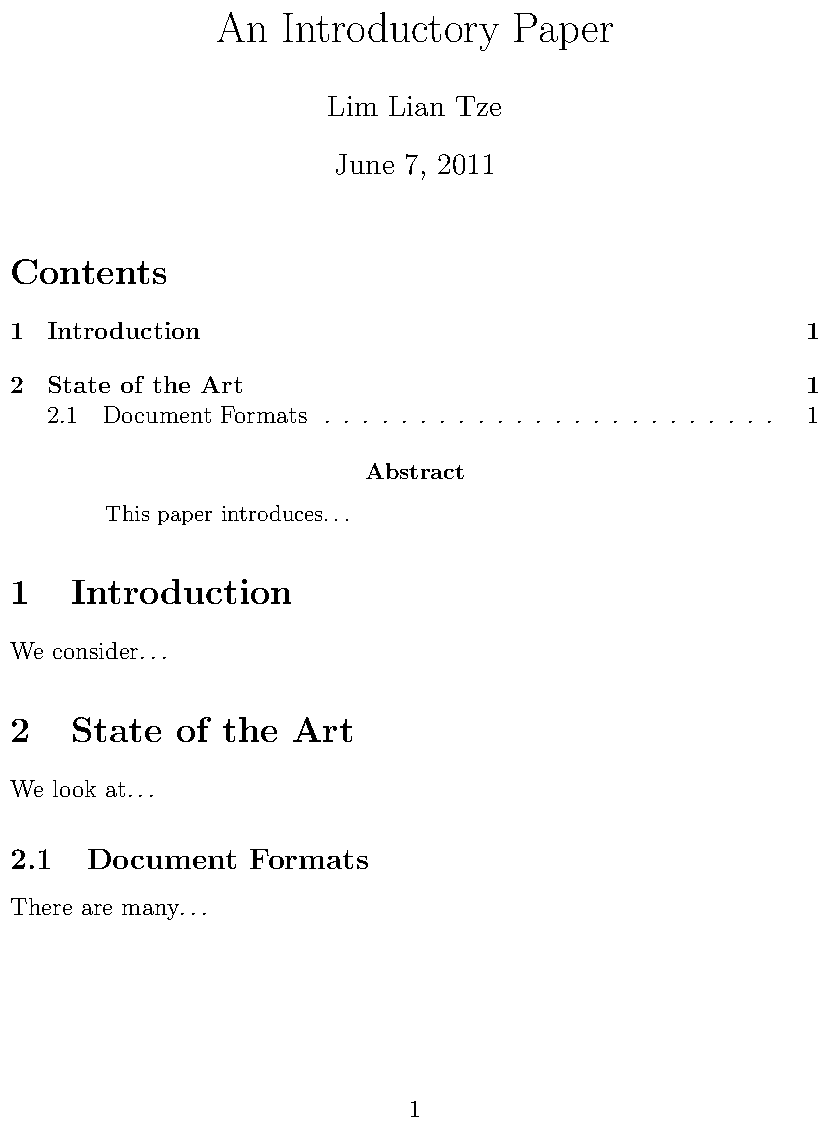
\includegraphics[width=.95\linewidth]{examples/first-en}}}%
\uncover<4|trans:0|handout:0>{\llap{\fcolorbox{black}{white}{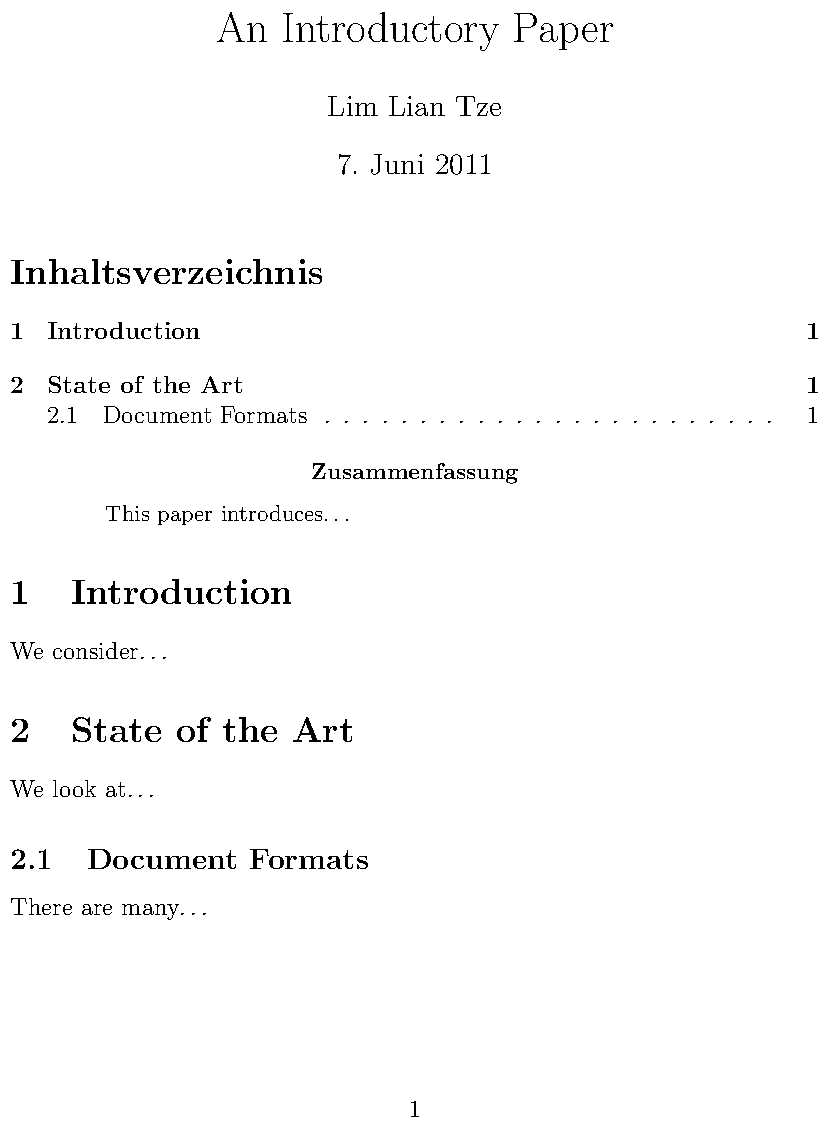
\includegraphics[width=.95\linewidth]{examples/first-de}}}}%
\uncover<5|trans:0|handout:0>{\llap{\fcolorbox{black}{white}{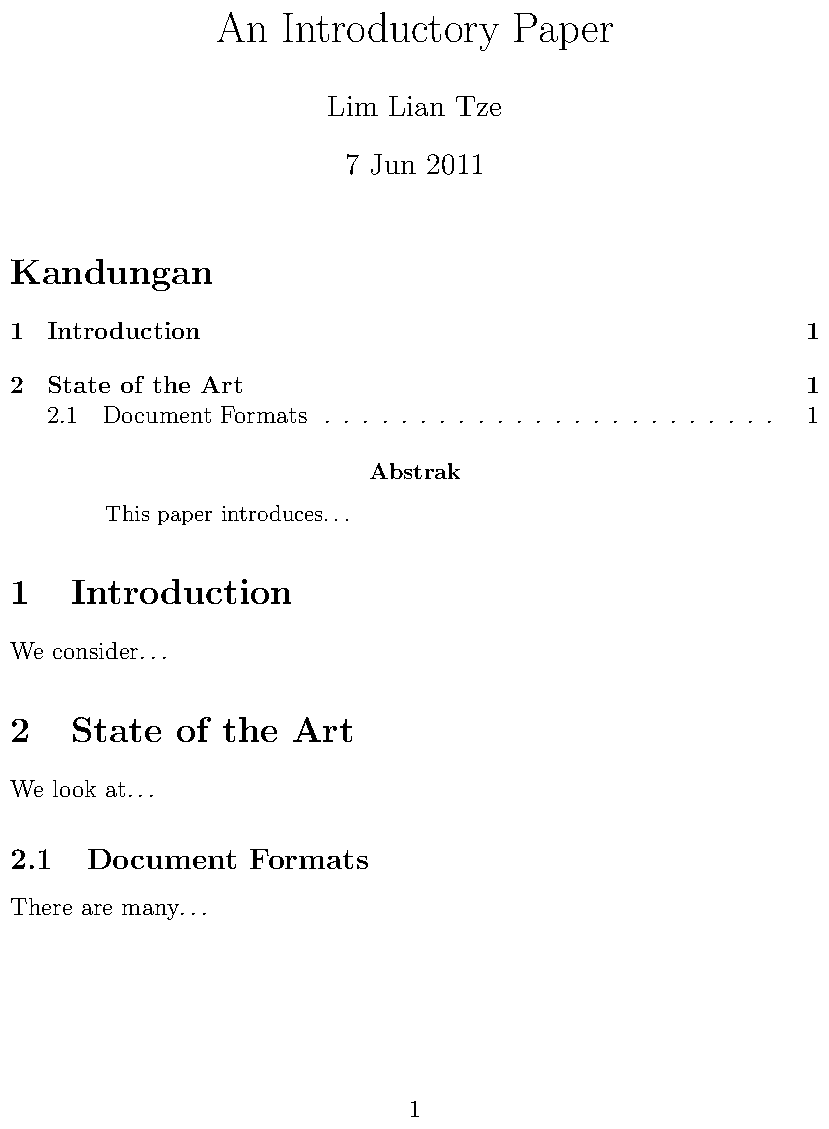
\includegraphics[width=.95\linewidth]{examples/first-ms}}}}
\end{column}
\end{columns}

\uncover<2->{\begin{tikzpicture}[remember picture,overlay]
\node[single arrow,fill=DarkSeaGreen,font=\ttfamily\bfseries,xshift=-1em] at (current page.center) {pdflatex};
\end{tikzpicture}
}

\end{frame}

\begin{frame}
\frametitle{Where Do I Get It?}
\begin{description}
\setlength\labelwidth{8.5em}
\setlength\itemindent{3em}
\item[Online] Overleaf (\url{www.overleaf.com})
\pause
\bigskip
\item[Windows] Mik\TeX, \TeX Live
\item[Un*x, \textsmaller{GNU}/Linux] \TeX Live
\item[Mac OS X] Mac\TeX\ (based on \TeX Live)
\item[Installation] Use your OS' package manager\\\hspace{\itemindent}(or download manually)
\pause
\item[Editors] vi, emacs, Texmaker, TeXworks, Texstudio, TeXshop\ldots
\pause
\item[\hologo{LaTeX} Packages] Use Mik\TeX\ or \TeX Live's package manager
\pause
\bigskip
\item[Documentation] 
{\small (Online)} \url{http://texdoc.net/pkg/<package name>}\\
\hspace{\itemindent}{\small (\TeX Live)} \texttt{\$ texdoc <package name>}\\
\hspace{\itemindent}{\small (Mik\TeX)} \texttt{\$ mthelp <package name>}
\end{description}
\end{frame}

\begin{frame}
\frametitle{Easy to Learn, Hard to Master}
\begin{itemize}
\item<+-> Customising may not be straightforward (vs word processors)
\item<+-> Intentionally so: Style guidelines should be followed strictly
\begin{itemize}
\item Publisher/organisation provides \structure{document class} or \structure{style} files
\item Use these to take care of formatting and styling, focus on the \structure{content}
\end{itemize}
% \item<+-> Fair enough. \\But where do I learn all the stuff the \TeX nicians do?
% \item<+-> (There \emph{is} a learning curve)
\end{itemize}
\end{frame}

\begin{frame}
\frametitle{Too hard, only for engineers/mathematicians?}

\begin{columns}[T]
\begin{column}{0.58\textwidth}
\begin{itemize}[<+->]
\item I once guided a student in the humanities to learn authoring Chinese \LaTeX{} documents entirely through e-mail
\item Recently a 75-year-old user transitioned to \LaTeX{} on Overleaf to write a book (with indices, end notes, cross references)
\item Professor in Finance at Trinity College transitioned to \LaTeX{} successfully (\url{https://www.overleaf.com/blog/299})
\item Linguists, psychologists, biostatistics (integrating with R), legal profession\ldots
\end{itemize}
\end{column}
\hfill
\begin{column}{.29\textwidth}<3->
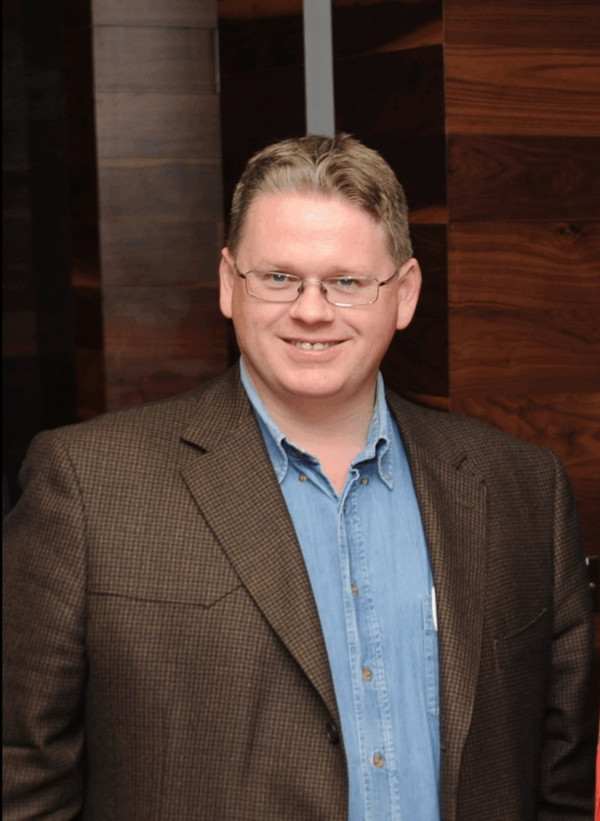
\includegraphics[width=\linewidth]{brian-lucey-full}\\
{\footnotesize Prof Brian Lucey, Trinity College, Dublin}
\end{column}
\end{columns}

\end{frame}

{\setbeamertemplate{background canvas}{\hskip-1.75em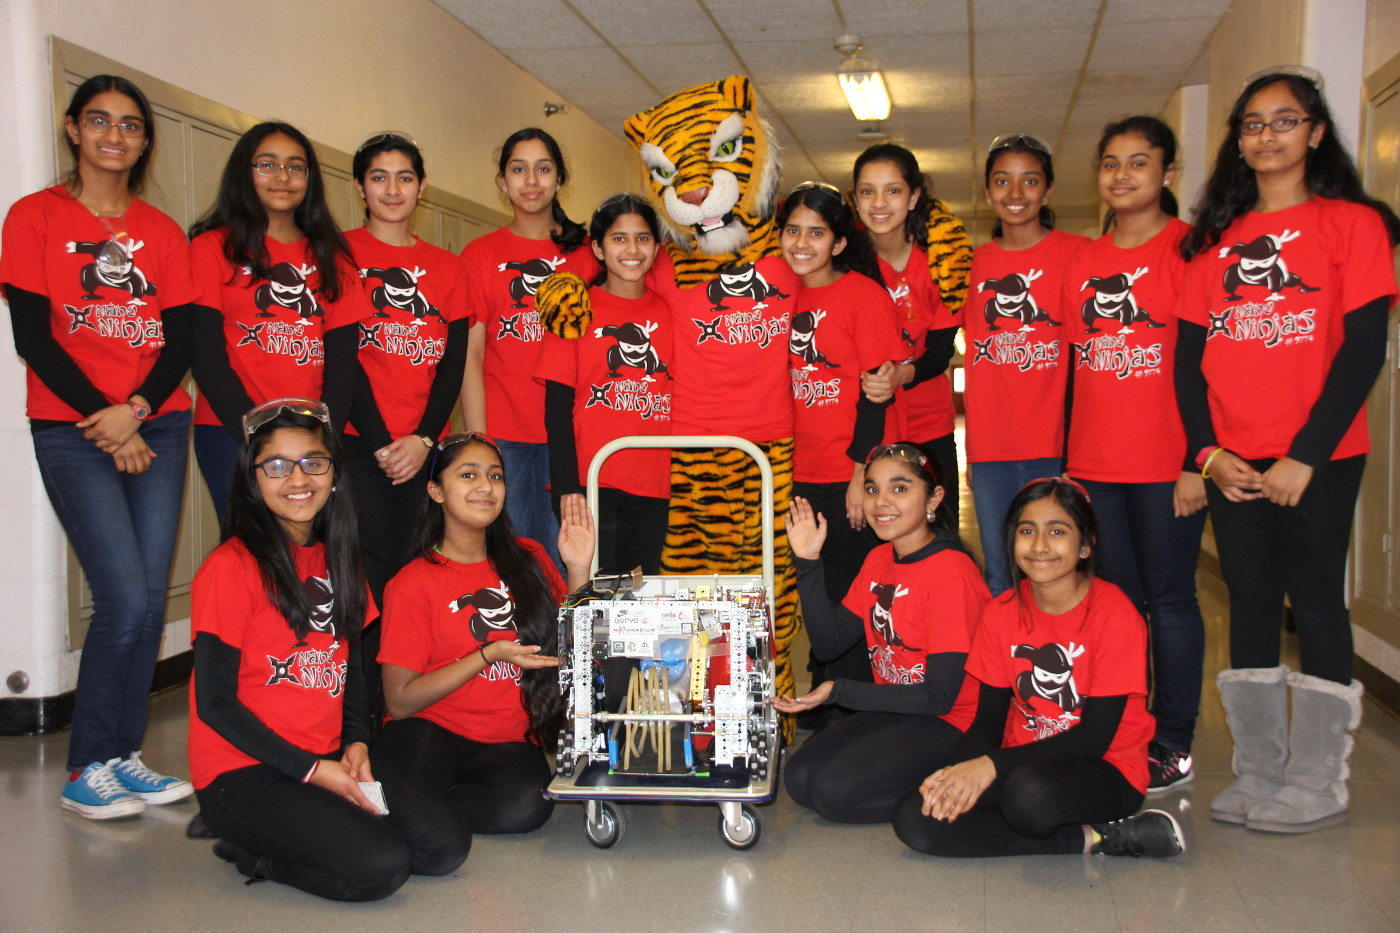
\includegraphics[height=\paperheight]{IMG_1710}}
\begin{frame}[plain,t]
\tikz\node[text=palette tertiary.fg,fill=palette tertiary.bg,opacity=0.8,font=\small\bfseries,text width=\textwidth,align=center]{Nano Ninjas -- a group of 7th- and 8th-graders from Portland, OR};

\vspace*{.87\textheight}

\tikz\node[text=palette tertiary.fg,fill=palette tertiary.bg,opacity=0.8,font=\footnotesize,text width=\textwidth,align=center]{Collaboratively wrote an engineering notebook with \textbf{300+ pages} in \LaTeX{} as part of their FIRST Tech Challenge win (\url{https://www.overleaf.com/read/hkxzqcncngyv})};
\end{frame}
}

\begin{frame}
\centering\Huge
So, What Can \hologo{LaTeX} Do?
\par
\end{frame}
% !TEX root=talk.tex

\section{Document Types}

\begin{frame}[fragile,allowframebreaks]
\frametitle{Basic Types}
\begin{columns}
\begin{column}{.35\textwidth}
\begin{beamerboxesrounded}[width=\linewidth]{Books}
\begin{lstlisting}[moretexcs={chapter,subsection,maketitle}, basicstyle={\ttfamily}, emph={book}]
\documentclass{book}
\author{...}
\title{...}

\begin{document}
\maketitle
\chapter{...}
\section{...}
...
\subsection{...}
\end{document}
\end{lstlisting}
\end{beamerboxesrounded}
\end{column}
\begin{column}{.58\textwidth}
\centering
\fcolorbox{black}{white}{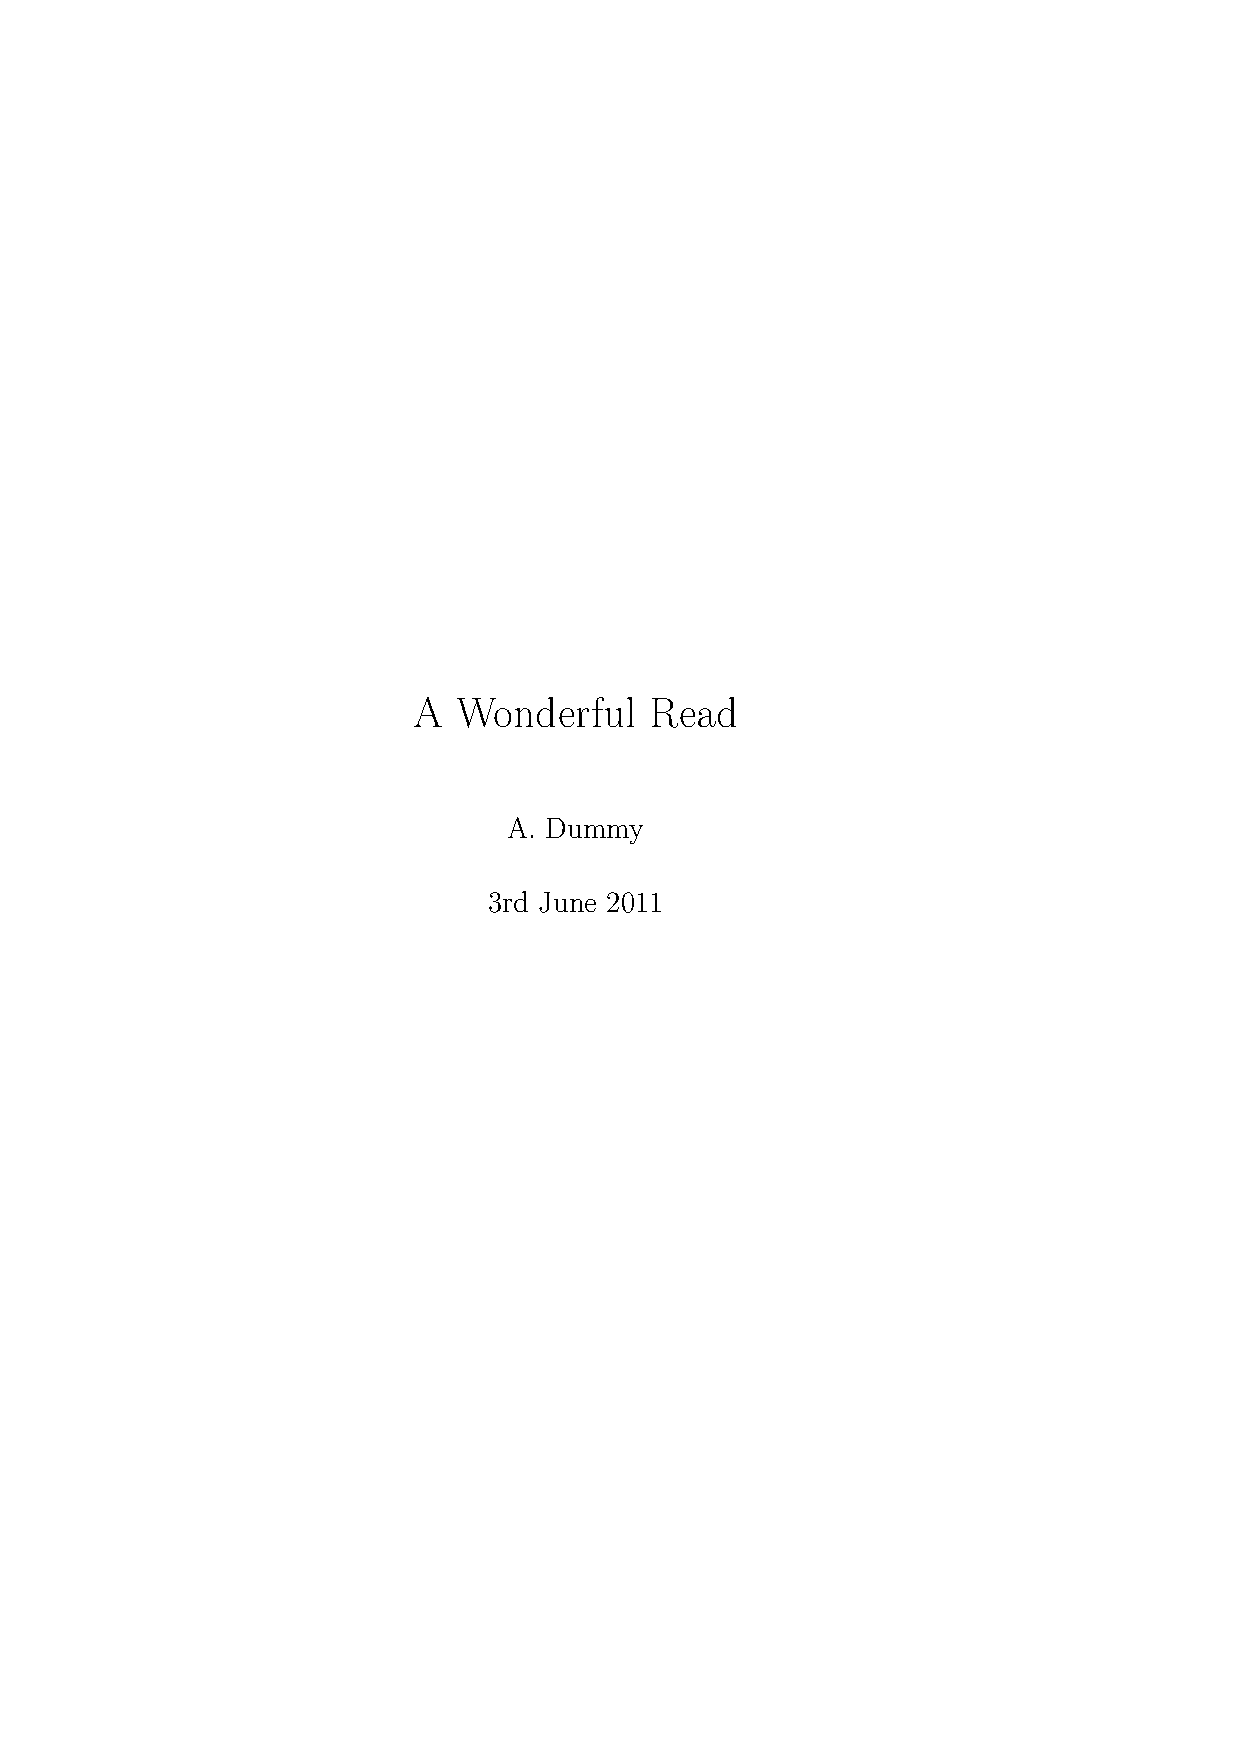
\includegraphics[width=.4\linewidth,page=1]{examples/basicbook}}
\fcolorbox{black}{white}{\includegraphics[width=.4\linewidth,page=3]{examples/basicbook}}
\fcolorbox{black}{white}{\includegraphics[width=.4\linewidth,page=4]{examples/basicbook}}
\fcolorbox{black}{white}{\includegraphics[width=.4\linewidth,page=5]{examples/basicbook}}
\end{column}
\end{columns}

\begin{columns}
\begin{column}{.4\textwidth}
\begin{beamerboxesrounded}[width=\linewidth]{Articles}
\begin{lstlisting}[moretexcs={chapter,subsection,maketitle}, basicstyle={\ttfamily}, emph={article}]
\documentclass{article}
\author{...}
\title{...}

\begin{document}
\maketitle
\section{...}
...
\subsection{...}
\end{document}
\end{lstlisting}
\end{beamerboxesrounded}
\end{column}
\begin{column}{.58\textwidth}
\centering
\fcolorbox{black}{white}{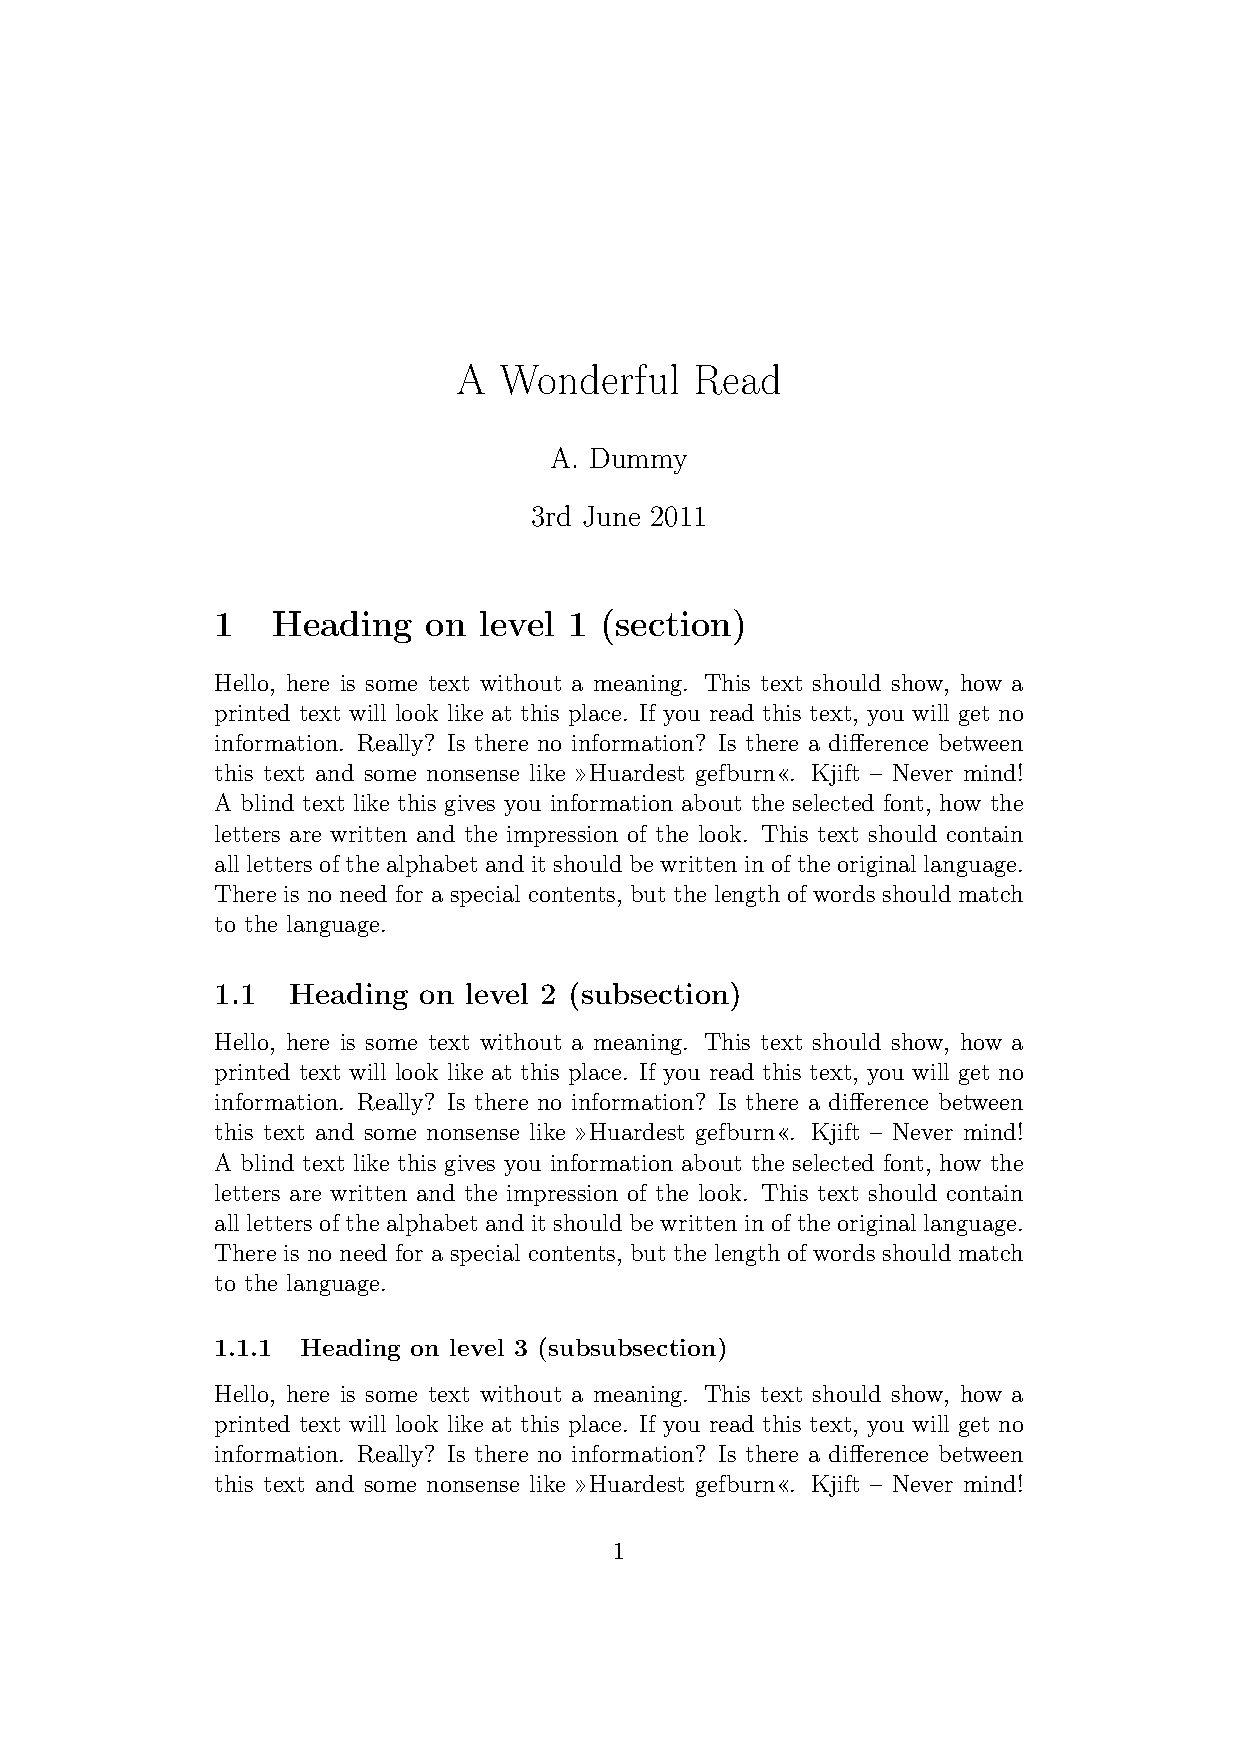
\includegraphics[width=.4\linewidth,page=1]{examples/basicarticle}}
\fcolorbox{black}{white}{\includegraphics[width=.4\linewidth,page=2]{examples/basicarticle}}
\fcolorbox{black}{white}{\includegraphics[width=.4\linewidth,page=3]{examples/basicarticle}}
\fcolorbox{black}{white}{\includegraphics[width=.4\linewidth,page=4]{examples/basicarticle}}
\end{column}
\end{columns}
\end{frame}

\begin{frame}[fragile]
\frametitle{Journal and Conference Proceedings Articles}
\begin{columns}[T]
\begin{column}{.33\textwidth}
\textsmaller{IEEE}\\\lstinline[basicstyle=\ttfamily\small]|\documentclass{IEEEtran}|
\vskip.5em
\fcolorbox{black}{white}{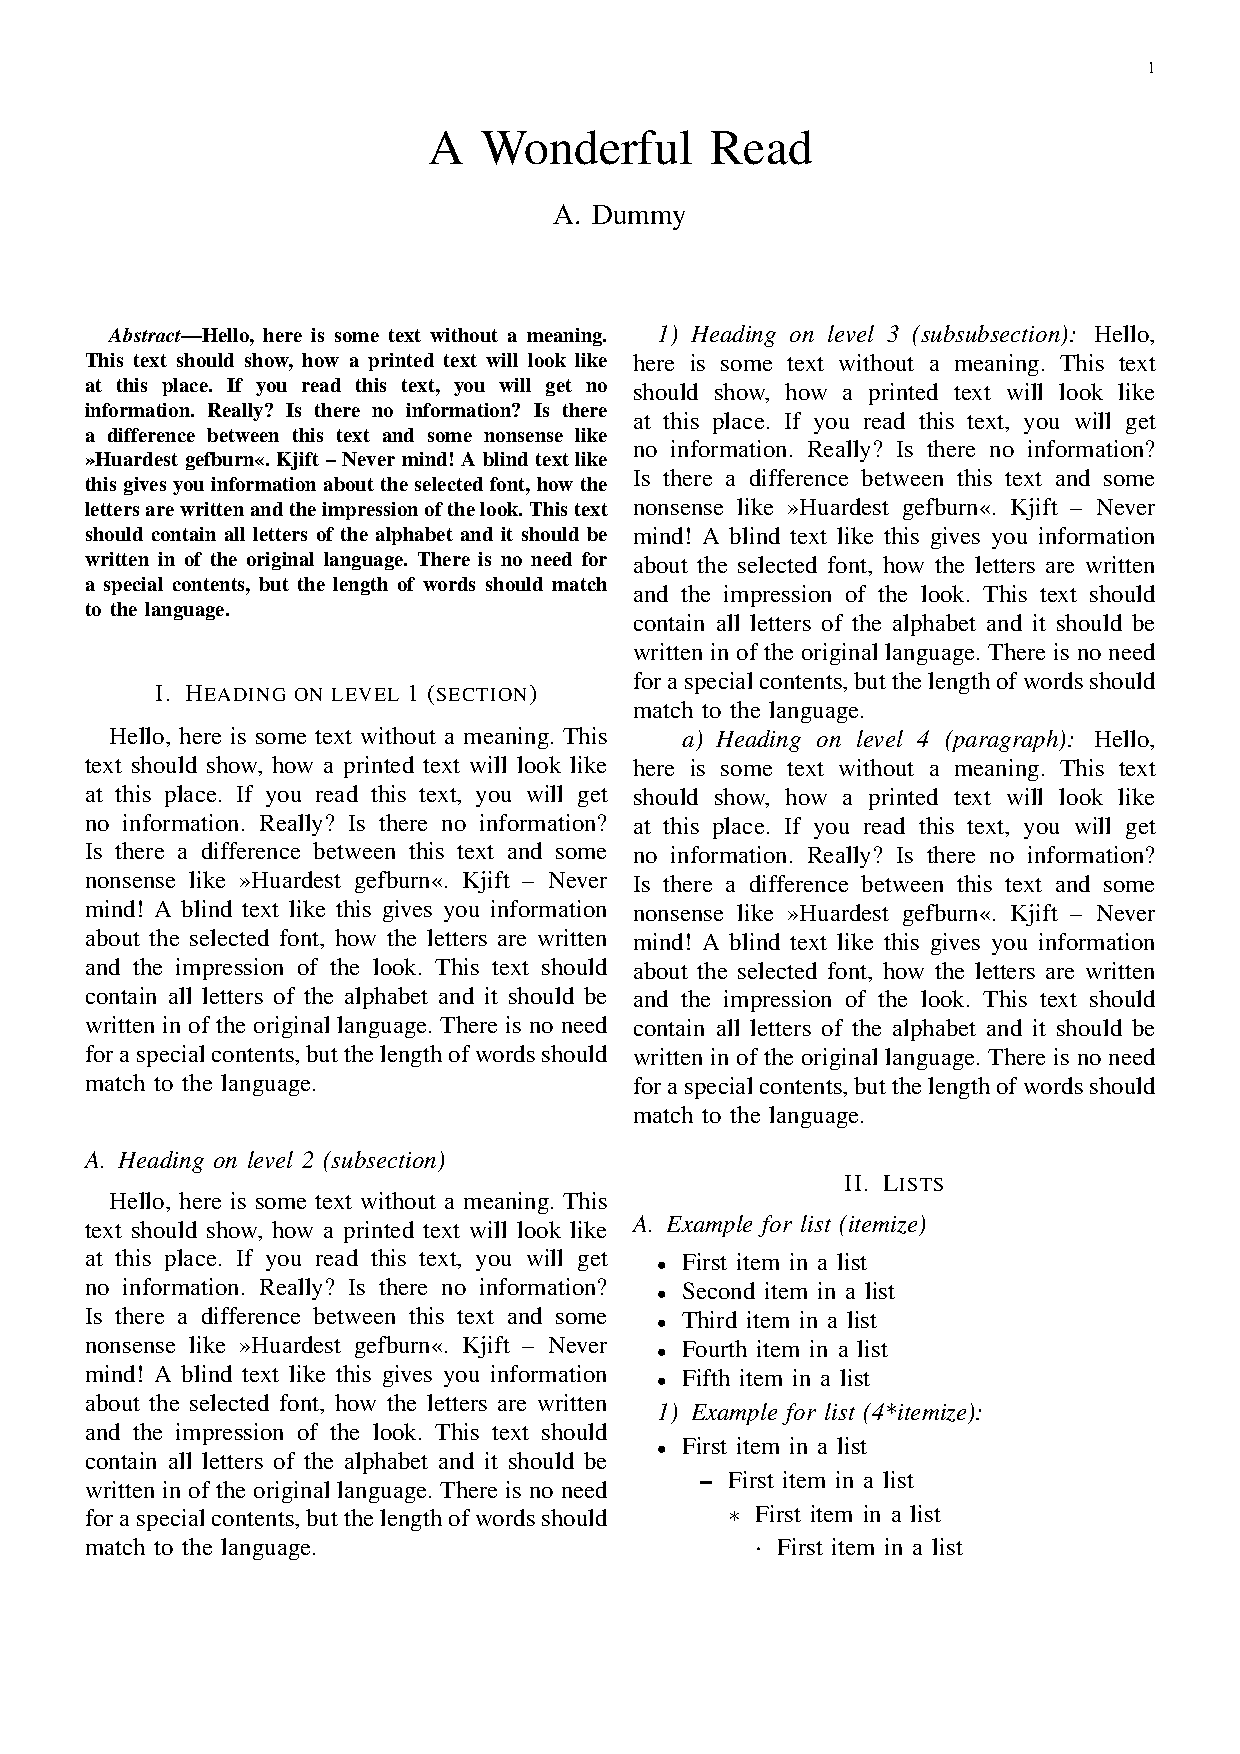
\includegraphics[width=\linewidth,page=1]{examples/IEEEtran}}
\end{column}

\begin{column}{.33\textwidth}
\textsmaller{ACM}\\\lstinline[basicstyle=\ttfamily\footnotesize\lsstyle,emphstyle=\scriptsize]|\documentclass{sig-alternate}|
\vskip.5em
\fcolorbox{black}{white}{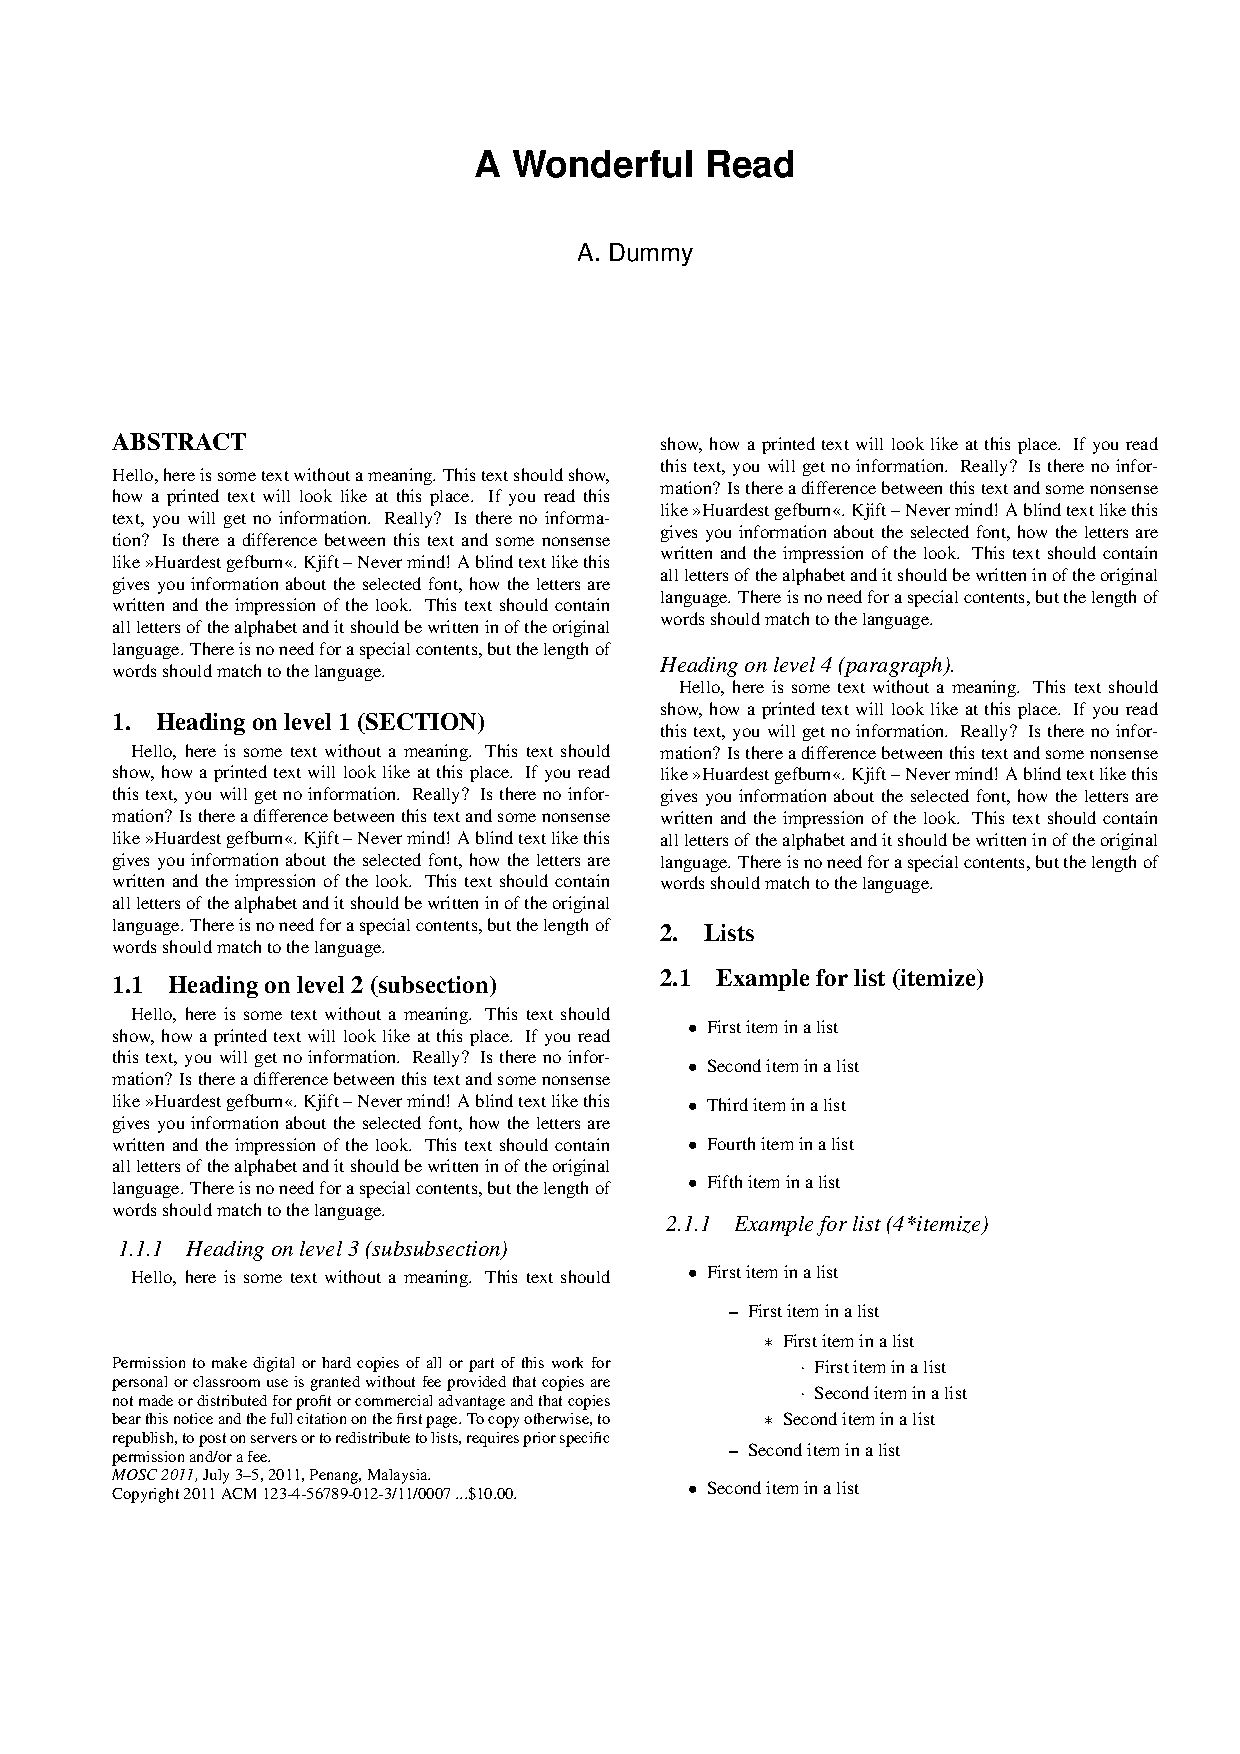
\includegraphics[width=\linewidth,page=1]{examples/acmconf}}
\end{column}

\begin{column}{.33\textwidth}
\textsmaller{LLNCS}\\\lstinline[basicstyle=\ttfamily\small]|\documentclass{llncs}|
\vskip.5em
\fcolorbox{black}{white}{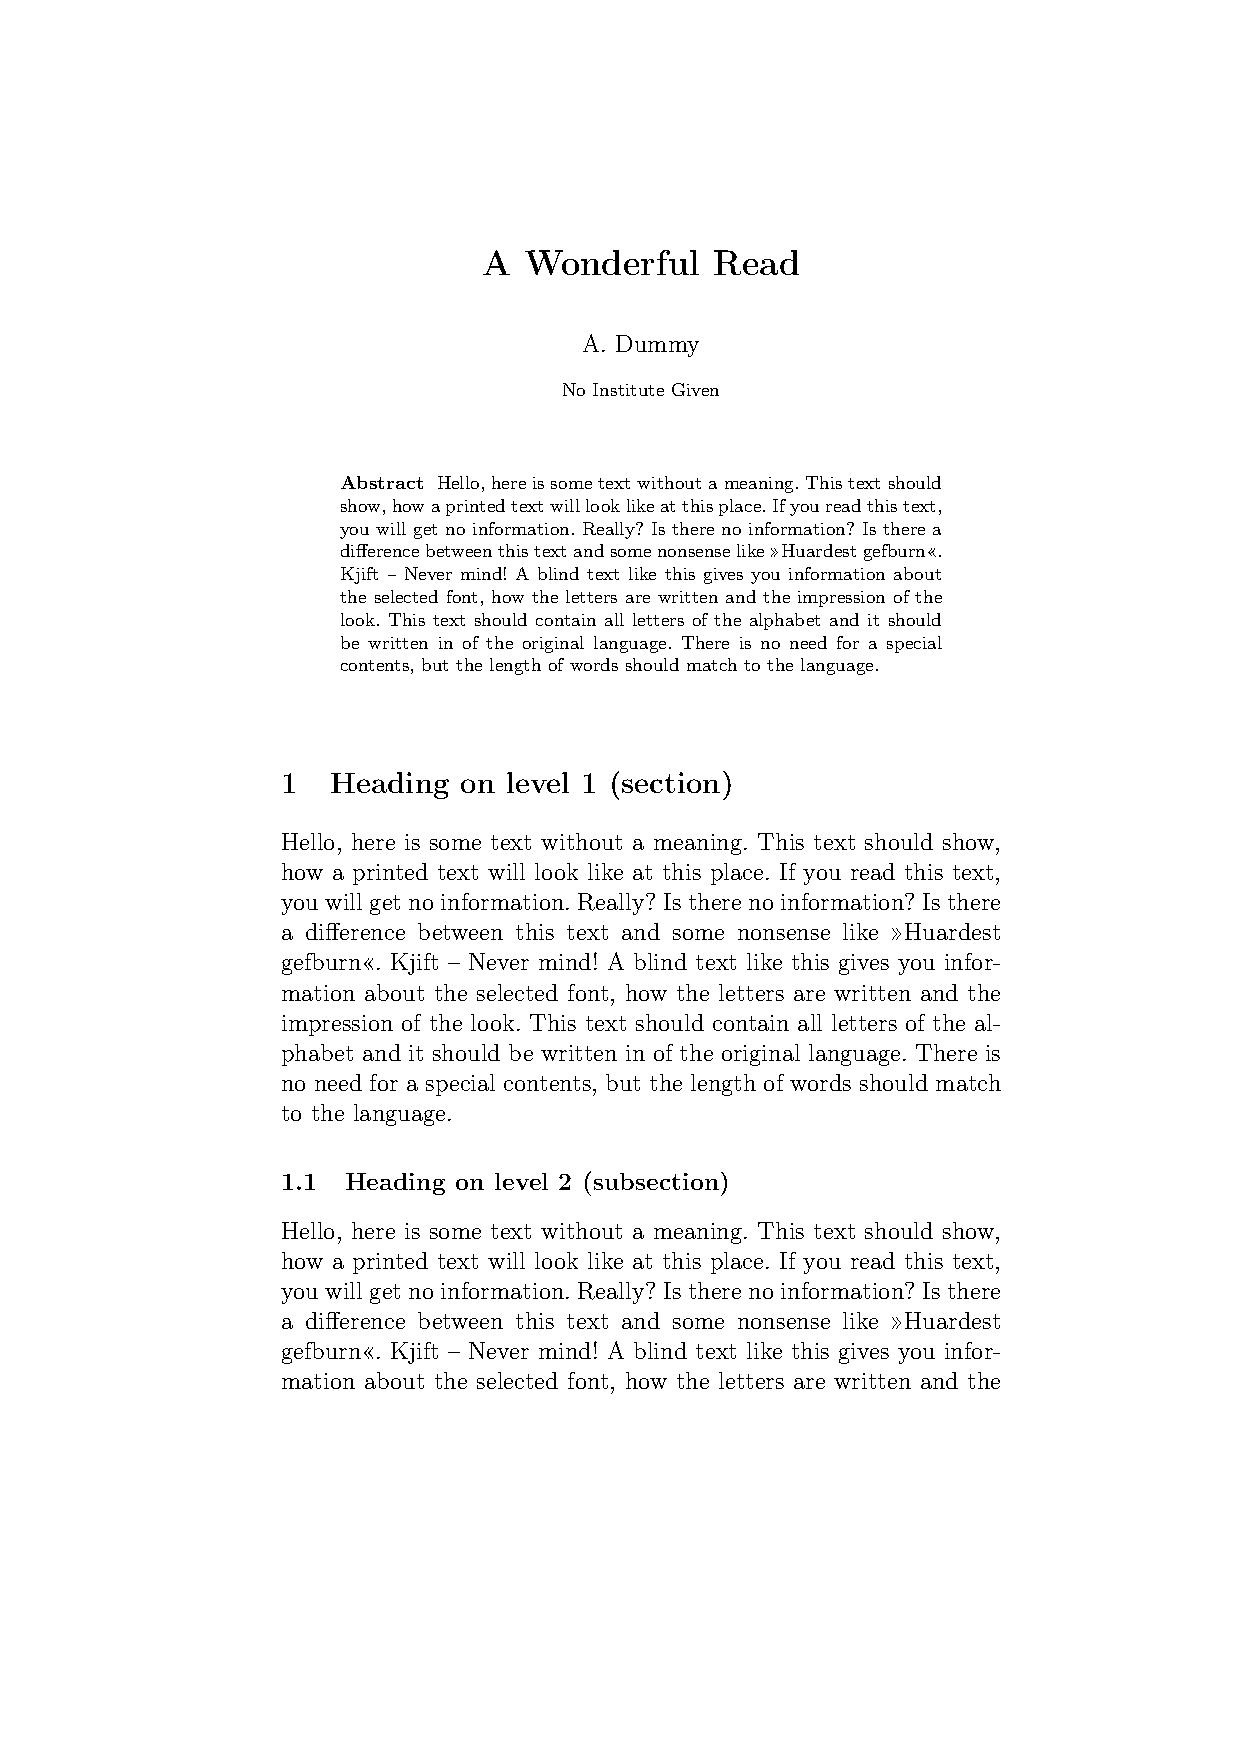
\includegraphics[width=\linewidth,page=1]{examples/llncs}}
\end{column}
\end{columns}
\end{frame}


\begin{frame}[fragile]
\lstset{basicstyle=\ttfamily}
\frametitle{Some Goodies}
\begin{itemize}
\item<+> Quick \structure{language-switching} with \texttt{babel}
\item<+> Automatic generation of \structure{cross-referencing labels}:\\
\lstinline|\section{Introduction}\label{sec:intro}|\\
\lstinline|... We saw in section \ref{sec:intro}...|
\item<+> Automatic generation of \structure{lists}:\\
\lstinline[texcs={tableofcontents}]|\tableofcontents|, \lstinline[texcs={listoffigures}]|\listoffigures|,  \lstinline[texcs={listoftables}]|\listoftables|
\item<+> Automatic generation of \structure{bibliographies} and \structure{indices}:\\
\lstinline|\cite{Knuth:1976}...\bibliography{references.bib}|\\
\lstinline[moretexcs={printindex}]|...the Linux kernel\index{Linux!kernel}... \printindex|\\
\item<+> Fully \structure{hyperlinked} \textsmaller{PDF} with bookmarks: \lstinline|\usepackage{hyperref}|
\item<+> Inclusion of selected pages from other \textsmaller{PDF}s\\(while inserting new page headers/footers!)\\
\lstset{basicstyle=\ttfamily\footnotesize,moretexcs={includepdf}}
\lstinline|\usepackage{pdfpages}|\\
\lstinline|\includepdf[pages={1,3-5,8},pagecommand=\thispagestyle{plain}]{file.pdf}|
\end{itemize}
\end{frame}

\begin{frame}
\frametitle{Multilingual \hologo{LaTeX}}
\centering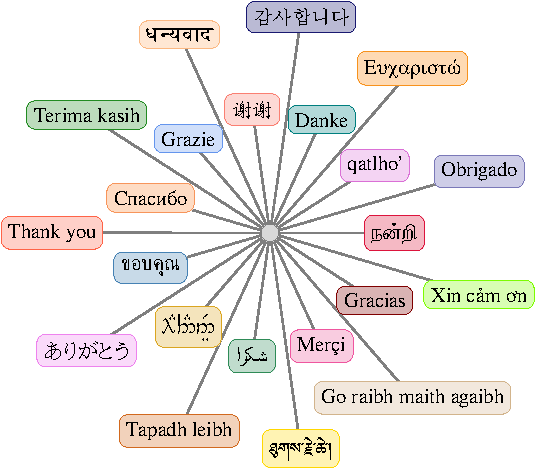
\includegraphics[height=.7\textheight]{multiling-TQ}\par
\pause
\begin{description}
\item[\hologo{XeLaTeX}, \hologo{LuaLaTeX}] Unicode input
\item[\hologo{LaTeX}] Various packages {\small (sometimes with transcriptions:  \texttt{nan\textasciicircum ri}, \texttt{salAm})}
\end{description}
\end{frame}

\begin{frame}[fragile,allowframebreaks]
\frametitle{University Theses}
\small
Universiti Sains Malaysia \lstinline[basicstyle=\ttfamily]|\documentclass{usmthesis}|
\vskip.5em

%% See http://liantze.penguinattack.org/latextypesetting.html#usmthesis
{\centering
\fcolorbox{black}{white}{\includegraphics[width=.24\linewidth,page=2]{examples/usmthesis.pdf}}
\fcolorbox{black}{white}{\includegraphics[width=.24\linewidth,page=4]{examples/usmthesis.pdf}}
\fcolorbox{black}{white}{\includegraphics[width=.24\linewidth,page=13]{examples/usmthesis.pdf}}
\fcolorbox{black}{white}{\includegraphics[width=.24\linewidth,page=36]{examples/usmthesis.pdf}}\par}

\mode<beamer>{
\pagebreak

%% See http://liantze.penguinattack.org/latextypesetting.html#mmuthesis
Multimedia University {\ttfamily{\color{Maroon}\bfseries\textbackslash documentclass}\{mmuthesis\}}
\vskip.5em

{\centering
\fcolorbox{black}{white}{\includegraphics[width=.24\linewidth,page=3]{examples/mmuthesis.pdf}}
\fcolorbox{black}{white}{\includegraphics[width=.24\linewidth,page=9]{examples/mmuthesis.pdf}}
\fcolorbox{black}{white}{\includegraphics[width=.24\linewidth,page=13]{examples/mmuthesis.pdf}}
\fcolorbox{black}{white}{\includegraphics[width=.24\linewidth,page=18]{examples/mmuthesis.pdf}}
\par}

\pagebreak

%% See http://liantze.penguinattack.org/latextypesetting.html#umalayathesis
Universiti Malaya {\ttfamily{\bfseries\color{Maroon}\textbackslash documentclass}\{umalayathesis\}}
\vskip.5em

{\centering
\fcolorbox{black}{white}{\includegraphics[width=.24\linewidth,page=2]{examples/umalayathesis.pdf}}
\fcolorbox{black}{white}{\includegraphics[width=.24\linewidth,page=6]{examples/umalayathesis.pdf}}
\fcolorbox{black}{white}{\includegraphics[width=.24\linewidth,page=12]{examples/umalayathesis.pdf}}
\fcolorbox{black}{white}{\includegraphics[width=.24\linewidth,page=20]{examples/umalayathesis.pdf}}
\par}}

\end{frame}


\begin{frame}
\frametitle{Highly Configurable Documents}
\framesubtitle{\texttt{memoir} and \textsmaller{KOMA}-Script Classes}

\begin{itemize}
\item Sectional headings
\item Running headers and footers
\item Good font, colour and illustration choices
\item \url{http://latex-my.blogspot.com/search/label/bookdesign}
\end{itemize}

%% See http://liantze.penguinattack.org/ebooks.html
\begin{center}
\onslide<2>{%
%\fcolorbox{black}{white}{\includegraphics[width=.24\linewidth,page=1]{examples/GridComputingCluster-Report2009}}
%\fcolorbox{black}{white}{\includegraphics[width=.24\linewidth,page=5]{examples/GridComputingCluster-Report2009}}
%\fcolorbox{black}{white}{\includegraphics[width=.24\linewidth,page=10]{examples/GridComputingCluster-Report2009}}
%\fcolorbox{black}{white}{\includegraphics[width=.24\linewidth,page=32]{examples/GridComputingCluster-Report2009}}
%}
\fcolorbox{black}{white}{
\includegraphics[width=.24\linewidth,page=1]{examples/GridBookExcerpt}}
\fcolorbox{black}{white}{
\includegraphics[width=.24\linewidth,page=2]{examples/GridBookExcerpt}}
\fcolorbox{black}{white}{
\includegraphics[width=.24\linewidth,page=3]{examples/GridBookExcerpt}}
\fcolorbox{black}{white}{\includegraphics[width=.24\linewidth,page=4]{examples/GridBookExcerpt}}
}
\end{center}
\end{frame}



\begin{frame}[fragile]
\frametitle{Presentation Slides}
\begin{itemize}
\item This presentation was made with \LaTeX!
\item<+-> Many possible classes: \texttt{powerdot}, \alert<2->{\texttt{beamer}}
\end{itemize}

\begin{columns}<+->
\begin{column}{.47\textwidth}
\begin{beamerboxesrounded}[width=\linewidth]{}
\vskip-1em
\begin{lstlisting}[basicstyle=\ttfamily\small,
moretexcs={usetheme,frametitle,frame,titleframe},
emph={beamer,frame},
escapechar={:},lineskip=-2pt]
\documentclass{beamer}
\usetheme{:\onslide<2>{Warsaw}%
\onslide<3|trans:0|handout:0>{\llap{Szeged}}%
\onslide<4|trans:0|handout:0>{\llap{Bergen}}%
\onslide<5|trans:0|handout:0>{\llap{oxygen}}%
\onslide<6|trans:0|handout:0>{\llap{Gelugor}}:}

\author ...

\begin{document}
\titleframe

\section{Intro}

\begin{frame}
\frametitle{Some Background}
...
:\bfseries\color{Maroon}\textbackslash end:{frame}
\end{document}
\end{lstlisting}
\vspace*{-1em}
\end{beamerboxesrounded}
\end{column}
\begin{column}{.48\textwidth}
\centering
\onslide<2>{\fcolorbox{black}{white}{\includegraphics[width=.7\linewidth,page=1]{examples/beamer-Warsaw}}}%
\onslide<3|trans:0|handout:0>{\llap{\fcolorbox{black}{white}{\includegraphics[width=.7\linewidth,page=1]{examples/beamer-Szeged}}
}}%
\onslide<4|trans:0|handout:0>{\llap{\fcolorbox{black}{white}{\includegraphics[width=.7\linewidth,page=1]{examples/beamer-Bergen}}
}}%
\onslide<5|trans:0|handout:0>{\llap{\fcolorbox{black}{white}{\includegraphics[width=.7\linewidth,page=1]{examples/beamer-Oxygen}}
}}%
\onslide<6|trans:0|handout:0>{\llap{\fcolorbox{black}{white}{\includegraphics[width=.7\linewidth,page=1]{examples/beamer-Gelugor}}
}}
\onslide<2>{\fcolorbox{black}{white}{\includegraphics[width=.7\linewidth,page=2]{examples/beamer-Warsaw}}}%
\onslide<3|trans:0|handout:0>{\llap{\fcolorbox{black}{white}{\includegraphics[width=.7\linewidth,page=2]{examples/beamer-Szeged}}
}}%
\onslide<4|trans:0|handout:0>{\llap{\fcolorbox{black}{white}{\includegraphics[width=.7\linewidth,page=2]{examples/beamer-Bergen}}
}}%
\onslide<5|trans:0|handout:0>{\llap{\fcolorbox{black}{white}{\includegraphics[width=.7\linewidth,page=2]{examples/beamer-Oxygen}}
}}%
\onslide<6|trans:0|handout:0>{\llap{\fcolorbox{black}{white}{\includegraphics[width=.7\linewidth,page=2]{examples/beamer-Gelugor}}
}}
\end{column}
\end{columns}
\end{frame}

\begin{frame}[fragile]
\frametitle{Oversized Posters}
\begin{itemize}
\item Many possible solutions:\\\texttt{sciposter}, \texttt{flowfram}, \alert<2-3>{\texttt{beamerposter}}, \alert<4-|trans:0|handout:0>{\texttt{tikzposter}}
\end{itemize}

% beamerposter
\begin{columns}<2-3>
\begin{column}{.5\textwidth}
\begin{beamerboxesrounded}[width=\linewidth]{}
\begin{lstlisting}[basicstyle=\ttfamily\small,
moretexcs={usetheme,frametitle,frame},
emph={beamer,beamerposter,frame},
escapechar={:},lineskip=-2pt]
\documentclass{beamer}
\usepackage[orientation=portrait, size=a0]{beamerposter}
\usetheme{...}
\author ... % Meta-information

\begin{document}
\begin{frame}
... % Poster contents goes here
:\bfseries\color{Maroon}\textbackslash end:{frame}
\end{document}
\end{lstlisting}
\end{beamerboxesrounded}
\end{column}
\begin{column}{.48\textwidth}
\centering
% See http://latex-my.blogspot.com/2011/03/creating-academic-posters-and-printing.html
\onslide<2>{\fcolorbox{black}{white}{\includegraphics[width=.8\linewidth]{examples/cicling-poster-small.pdf}}}%
\onslide<3|trans:0|handout:0>{\llap{\fcolorbox{black}{white}{\includegraphics[width=.8\linewidth]{examples/NLPCS08-poster-small}}
}}
\end{column}
\end{columns}

\onslide<4|trans:0|handout:0>{\vspace*{-.75\textheight}}

% tikzposter
\begin{columns}<4|trans:0|handout:0>
\begin{column}{.5\textwidth}
\begin{beamerboxesrounded}[width=\linewidth]{}
\begin{lstlisting}[basicstyle=\ttfamily\small,
moretexcs={usetheme,frametitle,frame},
emph={beamer,beamerposter,frame},
escapechar={:},lineskip=-2pt]
\documentclass[25pt,a1paper]{tikzposter}
\usetheme{Envelope} % nice themes!
\author ... % Meta-information

\begin{document}
... % Poster contents goes here
\end{document}
\end{lstlisting}
\end{beamerboxesrounded}
\end{column}
\begin{column}{.48\textwidth}
\centering
% See http://latex-my.blogspot.com/2011/03/creating-academic-posters-and-printing.html
\onslide<4>{\fcolorbox{black}{white}{\includegraphics[width=.8\linewidth]{examples/sample-tikzposter.pdf}}}%
\end{column}
\end{columns}

\end{frame}


\begin{frame}[fragile]
\frametitle{Leaflets}

\begin{itemize}
\item \texttt{leaflet}: arrange contents into 6 pages on a foldable double-sided sheet
\end{itemize}

\begin{columns}
\begin{column}{.496\textwidth}
\begin{beamerboxesrounded}[width=\linewidth]{}
\begin{lstlisting}[basicstyle=\ttfamily\small,lineskip=-2pt,emph={leaflet},moretexcs={maketitle}]
\documentclass[foldmark,a4paper]
{leaflet}
\author ... % Meta-information

\begin{document}
\maketitle
\section ...
... % Leaflet contents
\end{document}
\end{lstlisting}
\end{beamerboxesrounded}
\end{column}
\begin{column}{.48\textwidth}
\centering
% See http://latex-my.blogspot.com/2011/04/making-leaflets-with-l-t-e-x.html
\fcolorbox{black}{white}{\includegraphics[width=.85\linewidth,page=1]{examples/cicling-handout.pdf}}
\fcolorbox{black}{white}{\includegraphics[width=.85\linewidth,page=2]{examples/cicling-handout.pdf}}\par
\end{column}
\end{columns}

\end{frame}


\begin{frame}[fragile,allowframebreaks]
\frametitle{Fillable \textsmaller{PDF} Forms}
\begin{columns}
\begin{column}{.52\textwidth}
\begin{beamerboxesrounded}{}
\begin{lstlisting}[basicstyle=\ttfamily\small,escapechar=|,
moretexcs={TextField,ChoiceMenu,CheckBox},
emph={hyperref}]
\usepackage{hyperref}
... % various settings skipped
\TextField{Name:}\\
\TextField{Affiliation:}\\
\ChoiceMenu[radio=true]
{Are you a:}{Student, Academic}\\
Interest:
\CheckBox{Security}
\CheckBox{Systems}
\CheckBox{User space}\\
\TextField[multiline=true]
{Comments:}\\
\end{lstlisting}
\end{beamerboxesrounded}
\end{column}
\begin{column}{.47\textwidth}
\centering\includegraphics[width=\linewidth]{examples/form-screencap}\par
\end{column}
\end{columns}
\pagebreak

\alert{Use with caution!}
\begin{itemize}
\item \texttt{poppler}-based viewers (\texttt{evince}, \texttt{xpdf}, \texttt{okular})
\begin{itemize}
\item Problem displaying and saving radio/check boxes correctly
\item Saved forms can't be opened by other viewers
\end{itemize}
\item Adobe Reader
\begin{itemize}
\item Cannot save filled form as \textsmaller{PDF} unless Acrobat is installed
\item Only as field-and-value text file
\item Can provide ``Submit'' button for submission to a \textsmaller{URL}
\item Or print hard copy of filled form!
\end{itemize}
\item PDF XChange Viewer
\begin{itemize}
\item Best freeware for filling and saving \LaTeX-created forms
\item Windows only
\item Not \textsmaller{OSS}
\end{itemize}
\end{itemize}

\end{frame}


\begin{frame}[fragile]
\frametitle{Flash Cards}
\begin{columns}
\begin{column}{.465\textwidth}
\begin{beamerboxesrounded}{}
\vskip-1em
\begin{lstlisting}[basicstyle={\ttfamily\small},
emph={flashcards,flashcard},
moretexcs={cardfrontstyle,cardfrontfoot}]
\documentclass[avery5388,frame]
{flashcards}
\cardfrontstyle{headings}
\cardfrontfoot{Linux}

\begin{document}
\begin{flashcard}[Security]
{Certificate}
...
\end{flashcard}

\begin{flashcard}[Security]
{MAC ...}
...
\end{flashcard}
\end{document}
\end{lstlisting}
\vspace*{-1em}
\end{beamerboxesrounded}
\end{column}

\begin{column}{.53\textwidth}
\centering
\includegraphics[width=.49\linewidth,page=1]{examples/flashcard-crop}\hfill
\includegraphics[width=.49\linewidth,page=2]{examples/flashcard-crop}
\par
\end{column}
\end{columns}
\end{frame}


\begin{frame}[fragile]
\frametitle{Examination Paper}
\begin{columns}[T]
\begin{column}{.49\textwidth}
\begin{beamerboxesrounded}{}
\vskip-1em
\begin{lstlisting}[moretexcs={question,choice,CorrectChoice,part,printanswers},
emph={exam,questions,oneparchoices,parts,solution},
basicstyle=\ttfamily\scriptsize\lsstyle,lineskip=-1pt,escapechar=;]
\documentclass{exam}
...
\begin{questions};\onslide<2>{\bfseries\color{Maroon}\textbackslash printanswers};
\question[5] 
What is Paul McCartney's middle name?
\begin{oneparchoices}
\choice John \CorrectChoice Paul 
\choice Ringo \choice James
\end{oneparchoices}

\question[10] What was the Beatles' first single in 1962?
\begin{solution}Love Me Do\end{solution}

\question
\begin{parts} 
\part[5] What was George's inspiration for `While My Guitar Gently Weeps'?
\begin{solution}
He opened a random book and saw the words ``gently weep''.
\end{solution} 
...
\end{questions}
\end{lstlisting}
\vspace{-1em}
\end{beamerboxesrounded}
\end{column}
\begin{column}{.49\textwidth}
\centering
\onslide<1|trans:0|handout:0>{\fcolorbox{black}{white}{\includegraphics[width=\linewidth,page=1]{examples/exam}}}%
\onslide<2>{\llap{\fcolorbox{black}{white}{\includegraphics[width=\linewidth,page=2]{examples/exam}}}}
\end{column}
\end{columns}
\end{frame}

% \begin{frame}[fragile]
% \frametitle{KDU-exam}
% \begin{itemize}
% \item Automatic cover generation
% \item Automatic calculation of section marks, total marks, number of sections, number of pages
% \item Takes care of all formattings
% \end{itemize}

% \vspace*{-\baselineskip}
% \begin{columns}
% \begin{column}{.47\textwidth}
% \begin{beamerboxesrounded}{}
% \vskip-1em
% \begin{lstlisting}[moretexcs={coversubj,semester,examsection,droppoints,sectionpoints}]
% \coversubj{DIT1234 A Cool Subject}
% \semester{August 2013}
% ...

% \examsection{Basic Concepts}
% \begin{Questions}
% \Q[5] Give 5 examples. \droppoints
% \Q[8] Explain 4 concepts. \droppoints
% \end{Questions}
% \sectionpoints
% \end{lstlisting}
% \vspace{-1em}
% \end{beamerboxesrounded}
% \end{column}
% \begin{column}{.5\textwidth}
% \onslide<2>{\fcolorbox{black}{white}{\includegraphics[page=1,width=.8\textwidth]{sample}}}
% \onslide<3>{\llap{\fcolorbox{black}{white}{\includegraphics[page=2,width=.8\textwidth]{sample}}}}
% \end{column}
% \end{columns}

% \end{frame}
% !TEX root=talk.tex
\section{Special Material}

\begin{frame}[fragile]
\frametitle{Mathematics}
\begin{center}\begin{minipage}{.7\textwidth}\rmfamily
\eqref{eq:gratio} relates the golden ratio and the Fibonacci series.  Recall that the golden ratio, $\varphi = \frac{1}{2} (1 + \sqrt{5})$.

\begin{equation}\label{eq:gratio}
\varphi = 1 + \sum^{\infty}_{n=1}
                \frac{ (-1)^{n+1} }{ F_n F_{n+1} }
\end{equation}
\end{minipage}
\end{center}

\begin{beamerboxesrounded}{}
\vskip-1em
\begin{lstlisting}[escapechar=|,basicstyle=\ttfamily\small,moretexcs=eqref,emph={equation}]
\eqref{eq:gratio} relates the golden ratio and the Fibonacci series. 
Recall that the golden ratio, |\textcolor{red}{\large\ttfamily\$}|\phi = \frac{1}{2} (1 + \sqrt{5})|\textcolor{red}{\large\ttfamily\$}|.

\begin{equation}\label{eq:gratio}
\phi = 1 + \sum^{\infty} _{n=1}
                \frac{ (-1)^{n+1} }{ F_n F_{n+1} }
\end{equation}
\end{lstlisting}
\vspace*{-1em}
\end{beamerboxesrounded}
\end{frame}

\begin{frame}[fragile]
\frametitle{Chemical Equations and Molecules}

\begin{center}\rmfamily\small
\ce{Zn^2+ <=>[\ce{+ 2OH-}][\ce{+ 2H+}]
$\underset{\text{amphoteres Hydroxid}}{\ce{Zn(OH)2 v}}$
<=>C[+2OH-][{+ 2H+}]
$\underset{\text{Hydroxozikat}}{\cf{[Zn(OH)4]^2-}}$
}
\hfil
\chemfig{H-C(-[2]H)(-[6]H)-C(-[7]H)=[1]O}
\end{center}

\begin{beamerboxesrounded}{}
\vskip-1em
\begin{lstlisting}[basicstyle=\ttfamily\small,moretexcs={ce,chemfig,underset,text,cf},
emph={mhchem,chemfig}]
\usepackage[version=3]{mhchem}   % sufficient for chemical equations
\usepackage{chemfig}   % for 2-D molecule drawings
...
\ce{Zn^2+ <=>[\ce{+ 2OH-}][\ce{+ 2H+}]
$\underset{\text{amphoteres Hydroxid}}{\ce{Zn(OH)2 v}}$
<=> C[+2OH-][{+ 2H+}] 
$\underset{\text{Hydroxozikat}}{\cf{[Zn(OH)4]^2-}}$ }

\chemfig{H-C(-[2]H)(-[6]H)-C(-[7]H)=[1]O}
\end{lstlisting}
\vspace*{-1em}
\end{beamerboxesrounded}

\end{frame}

\begin{frame}[fragile]
\frametitle{Linguistics}

\begin{columns}[T]
\begin{column}{.54\textwidth}\small\rmfamily
\ex
\begingl
\gla \%*Wen liebt seine Mutter?//
\glb Whom loves his mother//
\glc `Who does his mother love?'//
\endgl
\xe

\begin{beamerboxesrounded}{}
\vskip-1em
\begin{lstlisting}[moretexcs={ex,xe,gla,glb,glc},basicstyle=\ttfamily\footnotesize\lsstyle,
emph={expex},
lineskip=-2pt,commentstyle={}]
\usepackage{linguex,qtree}
...
\ex
\begingl
\gla \%*Wen liebt seine Mutter?//
\glb Whom loves his mother//
\glc `Who does his mother love?'//
\endgl
\xe
\end{lstlisting}
\vskip-1em
\end{beamerboxesrounded}
\end{column}
\begin{column}{.45\textwidth}\footnotesize\rmfamily
\Tree [ .S [.NP [.Pron He ] ] [.VP [.V kicked ] [.NP [.Det the ] [.N ball ] ] ] ]

\medskip

\begin{beamerboxesrounded}{}
\vskip-1em
\begin{lstlisting}[moretexcs={ex,xe,gla,glb,glcTree},basicstyle=\ttfamily\footnotesize\lsstyle,
emph={expex,qtree},
lineskip=-2pt,commentstyle={}]
\usepackage{qtree}
...
\Tree [ .S [.NP [.Pron He ] ] [.VP [.V kicked ] [.NP [.Det the ] [.N ball ] ] ] ]
\end{lstlisting}
\vspace*{-1em}
\end{beamerboxesrounded}

\end{column}
\end{columns}

\end{frame}


\begin{frame}[fragile]
\frametitle{Program Listings}

\begin{columns}
\begin{column}{.5\textwidth}
\begin{beamerboxesrounded}{}
\vspace{-1em}
\begin{lstlisting}[basicstyle=\ttfamily\footnotesize,
emph={listings,lstlisting},moretexcs={color}]
\usepackage{listings,xcolor}
...
\begin{lstlisting}
[language=C,columns=fullflexible,
basicstyle=\ttfamily,
keywordstyle=\bfseries\color{red},
commentstyle=\sffamily\color{green},
stringstyle=\rmfamily\color{orange}]
#include <stdio.h>
/* 
 | Prints "hello world"
 */
int main(void)
{
    printf("hello, world\n");
    return 0;
}
:\bfseries\color{Maroon}\textbackslash end:{lstlisting}
\end{lstlisting}
\vspace{-1em}
\end{beamerboxesrounded}
\end{column}
\hfill\begin{column}{.46\textwidth}
\begin{lstlisting}[language=C,escapechar=~,lineskip=-2pt,
basicstyle=\ttfamily,
commentstyle=\upshape\sffamily\small\color{SeaGreen4},keepspaces=true,
keywordstyle=\bfseries\color{Maroon},stringstyle=\rmfamily\color{Sienna2}]
#include <stdio.h>

/* 
 | Prints "hello world"
 */
int main(void)
{
    printf("hello, world\n");
    return 0;
}
\end{lstlisting}
\end{column}
\end{columns}
\end{frame}

\begin{frame}[fragile]
\frametitle{Network Protocols}
\begin{columns}
\begin{column}{.505\textwidth}
\begin{beamerboxesrounded}{}
\vspace{-1em}
\begin{lstlisting}[basicstyle=\ttfamily\footnotesize,
moretexcs={bitheader,wordgroupr,bitbox,endwordgroupr,wordbox},
emph={bytefield,rightwordgroup}]
\usepackage{bytefield}
...
\begin{bytefield}{16} 
\bitheader{0,7,8,15} \\ 
\begin{rightwordgroup}{Header} 
\bitbox{4}{Tag} & \bitbox{12}{Mask} \\ 
\bitbox{8}{Source} & 
\bitbox{8}{Destination} 
\end{rightwordgroup} \\ 
\wordbox{3}{Data} 
\end{bytefield} 
\end{lstlisting}
\vspace{-1em}
\end{beamerboxesrounded}
\end{column}
\begin{column}{.49\textwidth}\rmfamily\small
\hfill\begin{bytefield}[bitwidth=.75em]{16}
\bitheader{0,7,8,15} \\ 
\begin{rightwordgroup}{Header} 
\bitbox{4}{Tag} & \bitbox{12}{Mask} \\ 
\bitbox{8}{Source} & \bitbox{8}{Destination} 
\end{rightwordgroup}\\ 
\wordbox{3}{Data} 
\end{bytefield} 
\end{column}
\end{columns}
\end{frame}

\begin{frame}[fragile]
\frametitle{Life Sciences}

\begin{texshade}{examples/AQPpro.MSF.txt}
\shadingmode{similar} 
\threshold[80]{50} 
\setends{1}{80..112} 
\hideconsensus 
\feature{top}{1}{93..93}{fill:$\downarrow$}{first case (see text)} 
\feature{bottom}{1}{98..98}{fill:$\uparrow$}{second case (see text)} 
\end{texshade}
\vskip-1em
\begin{beamerboxesrounded}{}
\vskip-1em
\begin{lstlisting}[
moretexcs={setends,shadingmode,threshold,hideconsensus,feature,downarrow,uparrow},
emph={texshade},
basicstyle=\ttfamily\small,lineskip=-2pt,escapechar=|]
\usepackage{texshade}  % for nucleotide and peptide alignments
...
\begin{texshade}{AQPpro.MSF.txt} 
\shadingmode{similar} 
\threshold[80]{50} 
\setends{1}{80..112} 
\hideconsensus 
\feature{top}{1}{93..93}{fill:$\downarrow$}{first case (see text)} 
\feature{bottom}{1}{98..98}{fill:$\uparrow$}{second case (see text)} 
\end{texshade} 
\end{lstlisting}
\vspace{-1em}
\end{beamerboxesrounded}
\end{frame}

\begin{frame}[fragile]
\frametitle{Circuits and SI Units}
\begin{columns}
\begin{column}{.49\textwidth}\rmfamily
\begin{circuitikz}[transform shape,scale=.9]
\draw (0,0) node[anchor=east] {B}  to[short, o-*] (1,0)    to[R=20<\ohm>, *-*] (1,2)
  to[R=10<\ohm>, v=$v_x$] (3,2) -- (4,2)
  to[ cI=$\frac{\si{\siemens}}{5} v_x$, *-*] (4,0) -- (3,0)  to[R=5<\ohm>, *-*] (3,2)
  (3,0) -- (1,0)   (1,2) to[short, -o] (0,2) node[anchor=east]{A}
;\end{circuitikz}
\end{column}
\begin{column}{.49\textwidth}
\begin{itemize}\rmfamily
\item \SI{3.45d4}{\square\volt\cubic\lumen\per\farad}
\item \SIlist[per-mode=symbol]{40;85;103}{\kilo\metre\per\hour}
\end{itemize}
\end{column}
\end{columns}

\medskip

\begin{beamerboxesrounded}{}
\vskip-1em
\begin{lstlisting}[basicstyle=\ttfamily\footnotesize,lineskip=-2pt,
moretexcs={draw,si,siemens,ohm,SI,SIlist,square,volt,cubic,lumen,per,farad,kilo,metre,hour},
emph={siunitx,circuitikz},emph={[2]{draw,node,to}}
]
\usepackage{siunitx}
\usepackage[siunitx]{circuitikz}
...
\begin{circuitikz}
\draw (0,0) node[anchor=east] {B}
  to[short, o-*] (1,0)    to[R=20<\ohm>, *-*] (1,2)
  to[R=10<\ohm>, v=$v_x$] (3,2) -- (4,2)
  to[ cI=$\frac{\si{\siemens}}{5} v_x$, *-*] (4,0) -- (3,0)
  to[R=5<\ohm>, *-*] (3,2)
  (3,0) -- (1,0)   (1,2) to[short, -o] (0,2) node[anchor=east]{A}
;\end{circuitikz}

\SI{3.45d4}{\square\volt\cubic\lumen\per\farad}
\SIlist[per-mode=symbol]{40;85;103}{\kilo\metre\per\hour}
\end{lstlisting}
\vspace{-1em}
\end{beamerboxesrounded}
\end{frame}

\begin{frame}[fragile]
\frametitle{Meh, What Good is That? Can't Use it Anywhere Else.}
Actually, you can.

\bigskip

\pause
\begin{beamerboxesrounded}{}
\vskip-1em
\begin{lstlisting}[moretexcs={PreviewEnvironment,texshade},basicstyle=\ttfamily,emph={preview}]
\usepackage[active,tightpage]{preview}
\PreviewEnvironment{texshade}
...
\begin{texshade}
...
\end{texshade}
\end{lstlisting}
\vspace{-1em}
\end{beamerboxesrounded}

\begin{itemize}
\item Run \texttt{pdflatex} $\rightarrow$ cropped \textsmaller{PDF} containing \emph{only} contents of \texttt{texshade}
\pause
\item ImageMagick: \verb|convert -depth 150 texshade.pdf texshade.png|
\pause
\item Multiple environments $\rightarrow$ multi-page \textsmaller{PDF} and multiple \textsmaller{PNG}s
\end{itemize}
\end{frame}

\begin{frame}[fragile]
\frametitle{Bar Codes}
%%% CAUTION!!! This takes a LOOONG time to compile if you're using pdflatex. I'm just going to load the already generated PDFs instead.

% \begin{pspicture}
% \psbarcode{MECARD:N:Malaysia Open Source Conference 2011;TEL:+60196085482;URL:http://www.mosc.my/;EMAIL:secretariat@mosc.my;ADR:Bayview Beach Resort, Baru Ferringgi Penang;NOTE:Malaysia Open Source Conference 2011 (MOSC2011);;}{eclevel=L width=0.75 height=0.75}{qrcode}
% \end{pspicture}\;
\includegraphics[page=1]{talk-pics}\;
% \begin{pspicture}
% \psbarcode[scalex=0.7,scaley=0.7]{9781860742712}{ includetext guardwhitespace }{ean13} 
% \end{pspicture}\;
\includegraphics[page=2]{talk-pics}\;
% \begin{pspicture}
% \psbarcode[scalex=0.7,scaley=0.7]{978-3-86541-114}{includetext guardwhitespace}{isbn} 
% \end{pspicture}\;\;
\includegraphics[page=3]{talk-pics}\;
% \begin{pspicture}
% \psbarcode[scalex=0.7,scaley=0.7]{^453^178^121^239}{ columns=2 rows=10}{pdf417}
% \end{pspicture}%
\includegraphics[page=4]{talk-pics}
\llap{\raisebox{0.45in}{\includegraphics[page=5]{talk-pics}%
% \begin{pspicture}
% \psbarcode[scalex=0.6,scaley=0.6]{LE28HS9Z}{includetext}{royalmail}
% \end{pspicture}
}}

\bigskip

\begin{beamerboxesrounded}{}
\vskip-1em
\begin{lstlisting}[moretexcs={psbarcode},escapechar=|,basicstyle=\ttfamily\footnotesize,
emph={pst-barcode},emph={[2]{qrcode,ean13,isbn,pdf417,royalmail,}},
alsoletter={1347-}
]
\usepackage{auto-pst-pdf}  % Needed if running pdflatex; must use option -shell-escape
\usepackage{pstricks,pst-barcode}
...
|\color{Maroon}\bfseries\textbackslash begin|{pspicture}
\psbarcode{MECARD:N:Malaysia Open Source Conference...}{eclevel=L}{qrcode}
\psbarcode{9781860742712}{includetext guardwhitespace}{ean13} 
\psbarcode{978-3-86541-114}{includetext guardwhitespace}{isbn} 
\psbarcode{LE28HS9Z}{includetext}{royalmail}
\psbarcode{^453^178^121^239}{columns=2 rows=10}{pdf417}
|\color{Maroon}\bfseries\textbackslash end|{pspicture} 
\end{lstlisting}
\vspace{-1em}
\end{beamerboxesrounded}
\end{frame}

\begin{frame}[fragile]
\frametitle{Graph Plots}

{\centering
\pgfplotsset{height=.75\textheight,width=.9\textwidth}
\begin{tikzpicture}[transform shape,scale=.7]
\begin{loglogaxis}[xlabel=Dof]
\addplot table[x=dof,y=L2] {examples/datafile.dat}; \addlegendentry{$L_2$};
\addplot table[x=dof,y=Lmax] {examples/datafile.dat}; \addlegendentry{$L_\text{max}$};
\end{loglogaxis} 
\end{tikzpicture}
\par}

\medskip

\begin{beamerboxesrounded}{}
\vskip-1em
\begin{lstlisting}[basicstyle=\ttfamily\footnotesize,
emph={pgfplots,tikzpicture,loglogaxis},
moretexcs={addplot, table, addlegendentry,text},lineskip=-2pt]
\usepackage{pgfplots}
...
\begin{tikzpicture}
\begin{loglogaxis}[xlabel=Dof]
\addplot table[x=dof,y=L2]{datafile.dat}; \addlegendentry{$L_2$};
\addplot table[x=dof,y=Lmax]{datafile.dat};  \addlegendentry{$L_\text{max}$};
\end{loglogaxis} 
\end{tikzpicture} 
\end{lstlisting}
\vspace{-1em}
\end{beamerboxesrounded}

\end{frame}

\begin{frame}[fragile]
\frametitle{Spreadsheets}
\framesubtitle{(Seriously, use a proper spreadsheet application for complex stuff.)}
\begin{center}\rmfamily\STautoround*{2}
\begin{spreadtab}{{tabular}{l rrr}}
@ Year ending Mar 31 & @2009 & @2008 & @2007\\\midrule
@ Revenue & 14580.2 & 11900.4 & 8290.3\\
@ Cost of sales & 6740.2 & 5650.1 & 4524.2\\\cmidrule{2-4}
@\emph{Gross profit} & \STcopy{>}{b2-b3} & &\\\cmidrule[\lightrulewidth]{2-4}
\end{spreadtab}
\end{center}

\begin{beamerboxesrounded}{}
\vskip-1em
\begin{lstlisting}[basicstyle=\ttfamily\small,moretexcs={STcopy,STautoround*},
alsoletter={23->}, emph={spreadtab},
emph={[2]{b2-b3,>}}]
\STautoround*{2}
\begin{spreadtab}{{tabular}{l rrr}}
@Year ending Mar 31 & @2009 & @2008 & @2007\\ \hline
@Revenue & 14580.2 & 11900.4 & 8290.3\\
@Cost of sales & 6740.2 & 5650.1 & 4524.2\\ \cline{2-4}
@\emph{Gross profit} & \STcopy{>}{b2-b3} & &\\ \cline{2-4}
\end{spreadtab}
\end{lstlisting}
\vspace{-1em}
\end{beamerboxesrounded}

\end{frame}

\begin{frame}[fragile]
\frametitle{Gantt Charts}

\scalebox{.85}{\rmfamily
\begin{ganttchart}%
[y unit title=0.4cm,
y unit chart=0.5cm,
vgrid=true,
title/.style={draw=none, fill=RoyalBlue!50!black},
title label font=\sffamily\bfseries\color{white}, title label anchor/.style={below=-1.6ex},
title left shift=.05,
title right shift=-.05,
title height=1,
bar/.style={draw=none, fill=OliveGreen!75},
bar height=.6,
bar label font=\normalsize\color{black!50},
group right shift=0,
group top shift=.6,
group height=.3, group peaks height=.2,
bar incomplete/.style={fill=Maroon}]{1}{16} 
\gantttitle{2010}{4} \gantttitle{2011}{12} \\ 
\ganttbar%
[progress=100, bar progress label font=\small\color{OliveGreen!75}, progress label anchor/.style={right=4pt},
bar label font=\normalsize\color{OliveGreen},
name=pp]%
  {Preliminary Project}{1}{4} \\
\ganttset{progress label text={}, link/.style={black, -to}}
\ganttgroup{Objective 1}{5}{16} \\
\ganttbar[progress=4, name=T1A]{Task A}{5}{10} \\
\ganttlinkedbar[progress=0]{Task B}{11}{16} \\
\ganttgroup{Objective 2}{5}{16} \\
\ganttbar[progress=15, name=T2A]{Task A}{5}{13} \\
\ganttlinkedbar[progress=0]{Task B}{14}{16}
\end{ganttchart}
}

\begin{beamerboxesrounded}{}
\vskip-1em
\begin{lstlisting}[basicstyle=\ttfamily\footnotesize,lineskip=-2pt,
moretexcs={gantttitle,ganttbar,ganttlink,ganttgroup,ganttlinkedbar},
emph={pgfgantt,tikzpicture,ganttchart}]
\usepackage{pgfgantt}
...
\begin{ganttchart}[...settings...]{1}{16} 
\gantttitle{2010}{4} \gantttitle{2011}{12} \\ 
\ganttbar[progress=100]{Preliminary Project}{1}{4} \\ 
\ganttgroup{Objective 1}{5}{16} \\ 
\ganttbar[progress=4, name=T1A]{Task A}{5}{10} \\ 
\ganttlinkedbar[progress=0]{Task B}{11}{16} \\ 
...
\end{ganttchart} 
\end{lstlisting}
\vspace{-1em}
\end{beamerboxesrounded}

\end{frame}

\begin{frame}[fragile]
\frametitle{`Smart Diagrams'}
\begin{columns}[T]

\begin{column}{.49\textwidth}
\resizebox{\linewidth}{!}{\smartdiagram[bubble diagram]{Planning Cycle,Assess,Plan,Implement,Renew}}

\begin{beamerboxesrounded}{}
\vskip-1em
\begin{lstlisting}[basicstyle=\ttfamily\footnotesize,lineskip=-2pt]
\usepackage{smartdiagram}
\smartdiagram[bubble diagram]{
  Planning Cycle,Assess,Plan,
  Implement,Renew}
\end{lstlisting}
\vspace{-1em}
\end{beamerboxesrounded}
\end{column}

\begin{column}{.49\textwidth}
\resizebox{\linewidth}{!}{\smartdiagram[priority descriptive diagram]{Assess,Plan,Implement,Renew}}

\begin{beamerboxesrounded}{}
\vskip-1em
\begin{lstlisting}[basicstyle=\ttfamily\footnotesize,lineskip=-2pt]
\usepackage{smartdiagram}
\smartdiagram
  [priority descriptive diagram]{
  Assess,Plan,Implement,Renew}
\end{lstlisting}
\vspace{-1em}
\end{beamerboxesrounded}
\end{column}

\end{columns}

% \resizebox{\linewidth}{\smartdiagram[priority descriptive diagram]{Planning Cycle,Assess,Plan,Implement,Renew}}
\end{frame}

\begin{frame}[fragile]
\frametitle{Chess games}

\begin{columns}
\begin{column}{.51\textwidth}

\begin{beamerboxesrounded}{}
\vskip-1em
\begin{lstlisting}[basicstyle=\ttfamily\small,
moretexcs={newgame,mainline,chessboard},
emph={skak,chessboard}]
\usepackage[skaknew]%
{skak,chessboard}
...
\newgame
\mainline{1. e4 e5 2. Nf3 Nc6 3. Bb5 a6}
\chessboard[smallboard]
\end{lstlisting}
\vspace{-1em}
\end{beamerboxesrounded}
\end{column}

\begin{column}{.47\textwidth}
\rmfamily
\newgame\mainline{1. e4 e5 2. Nf3 Nc6 3. Bb5 a6}

\chessboard[smallboard]

\end{column}
\end{columns}
\end{frame}

\begin{frame}[fragile]
\frametitle{Crossword Puzzles}
\begin{columns}
\begin{column}{.3\textwidth}\rmfamily
\begin{Puzzle}{5}{3}
|* |* |[1]E|X |* |.
|[2]A|[3]S|T |* |[4]T|.
|* |[5]P|A |R |T |.
\end{Puzzle}
\end{column}
\begin{column}{.65\textwidth}\rmfamily
\begin{PuzzleClues}{
\textbf{Across:} }
  \Clue{1}{EX}{unit of measure}
  \Clue{2}{AST}{\(\ast\)}
  \Clue{5}{PART}{sectioning unit}
\end{PuzzleClues}
\begin{PuzzleClues}{
\textbf{Down:} }
  \Clue{1}{ETA}{\(\eta\)}
  \Clue{3}{SP}{unit of measure}
  \Clue{4}{TT}{nonproportional font}
\end{PuzzleClues}
\end{column}
\end{columns}

\begin{beamerboxesrounded}{}
\vskip-1em
\begin{multicols}{2}
\begin{lstlisting}[escapechar=?,basicstyle=\ttfamily\footnotesize,
moretexcs={Clue},emph={cwpuzzle,Puzzle,PuzzleClues}]
\usepackage{cwpuzzle}
...
\begin{Puzzle}{5}{3}
|* |* |[1]E|X |* |.
|[2]A|[3]S|T |* |[4]T|.
|* |[5]P|A |R |T |.
\end{Puzzle}
\begin{PuzzleClues}{
\textbf{Across:} }
  \Clue{1}{EX}{unit of measure}
  \Clue{2}{AST}{\(\ast\)}
  \Clue{5}{PART}{sectioning unit}
\end{PuzzleClues}
\begin{PuzzleClues}{
\textbf{Down:} }
  \Clue{1}{ETA}{\(\eta\)}
  \Clue{3}{SP}{unit of measure}
  \Clue{4}{TT}{nonproportional font}
\end{PuzzleClues}
\end{lstlisting}
\end{multicols}
\vspace{-.5em}
\end{beamerboxesrounded}
\end{frame}

\begin{frame}[fragile]
\frametitle{Song Books with Guitar Tabs}
\vskip-.55\textheight
\begin{guitar}
\rmfamily\smallchords\def\chordsize{.5em}
\renewcommand\yoff{2}
\renewcommand\xoff{0}
\renewcommand\namefont{\footnotesize\sffamily}
\renewcommand\normalsiz{1.1}
\renewcommand\topfretsiz{1.2pt}
\newcommand{\CMaj}{\chord{t}{n,p3,p2,n,p1,n}{C}}
\newcommand{\Amin}{\chord{t}{n,n,p2,p2,p1,n}{Am}}
\newcommand{\FMaj}{\chord{t}{n,n,p3,p2,p1,p1}{F}}
\newcommand{\GMaj}{\chord{t}{p3,p2,n,n,n,p3}{G}}
Country [\CMaj]road, take me [\GMaj]home, to the [\Amin]place I be[\FMaj]long.
West Vir[\CMaj]ginia, mountain [\GMaj]momma, take me [\FMaj]home, country [\CMaj]road.
\end{guitar}

\begin{beamerboxesrounded}{}
\vskip-1em
\begin{lstlisting}[moretexcs={chord,CMaj,Amin,FMaj,GMaj},
emph={gchords,guitar},
basicstyle=\ttfamily\small]
\usepackage{gchords,guitar}
...
\begin{guitar}
\newcommand{\CMaj}{\chord{t}{n,p3,p2,n,p1,n}{C}}
\newcommand{\Amin}...
Country [\CMaj]road, take me [\GMaj]home, ...
\end{guitar}
\end{lstlisting}
\vspace{-1em}
\end{beamerboxesrounded}
\end{frame}



\section{Wrapping Up}

\begin{frame}
\frametitle{Summary}
\begin{itemize}
\item<+-> \LaTeX
	\begin {itemize}
	\item a document preparation system
	\item professional quality typesetting output
	\end{itemize}
\item<+-> Output artefacts
	\begin{itemize}
	\item Academic: papers, theses, books
	\item Dedicated document types
	\item Domain-specific material
	\end{itemize}
\item<+-> Usage scenario
	\begin{itemize}
	\item Direct authoring
	\item Automatic generation (via scripts etc)
	\item As back-end of other applications
	\end{itemize}
\end{itemize}
\end{frame}

\begin{frame}
\centering
\includegraphics[width=.6\textwidth]{multiling-TQ}

\bigskip 
\begin{tabular}{cl}
\multirow{2}{*}{\huge Questions?} & \url{liantze@gmail.com}, \url{support@overleaf.com}\\
& \url{http://tex.stackexchange.com}\\
\end{tabular}

% {\huge Questions?\par}\vskip1em
% {\large\url{liantze@gmail.com}
% \\\url{support@overleaf.com}
% \\\url{http://liantze.penguinattack.org}
% \\\url{http://latex-my.blogspot.com}
% \par}
\end{frame}

\begin{frame}
\frametitle{Want to download this deck?}
\centering
\qrcode[height=.5\textheight]{https://www.overleaf.com/read/cyfvvyfrpmyn}
\end{frame}

\end{document}
